\documentclass[]{book}
\usepackage{lmodern}
\usepackage{amssymb,amsmath}
\usepackage{ifxetex,ifluatex}
\usepackage{fixltx2e} % provides \textsubscript
\ifnum 0\ifxetex 1\fi\ifluatex 1\fi=0 % if pdftex
  \usepackage[T1]{fontenc}
  \usepackage[utf8]{inputenc}
\else % if luatex or xelatex
  \ifxetex
    \usepackage{mathspec}
  \else
    \usepackage{fontspec}
  \fi
  \defaultfontfeatures{Ligatures=TeX,Scale=MatchLowercase}
\fi
% use upquote if available, for straight quotes in verbatim environments
\IfFileExists{upquote.sty}{\usepackage{upquote}}{}
% use microtype if available
\IfFileExists{microtype.sty}{%
\usepackage{microtype}
\UseMicrotypeSet[protrusion]{basicmath} % disable protrusion for tt fonts
}{}
\usepackage[margin=1in]{geometry}
\usepackage{hyperref}
\hypersetup{unicode=true,
            pdftitle={Machine Learning},
            pdfauthor={Mohamad Ghassany},
            pdfborder={0 0 0},
            breaklinks=true}
\urlstyle{same}  % don't use monospace font for urls
\usepackage{natbib}
\bibliographystyle{apalike}
\usepackage{color}
\usepackage{fancyvrb}
\newcommand{\VerbBar}{|}
\newcommand{\VERB}{\Verb[commandchars=\\\{\}]}
\DefineVerbatimEnvironment{Highlighting}{Verbatim}{commandchars=\\\{\}}
% Add ',fontsize=\small' for more characters per line
\usepackage{framed}
\definecolor{shadecolor}{RGB}{248,248,248}
\newenvironment{Shaded}{\begin{snugshade}}{\end{snugshade}}
\newcommand{\KeywordTok}[1]{\textcolor[rgb]{0.13,0.29,0.53}{\textbf{{#1}}}}
\newcommand{\DataTypeTok}[1]{\textcolor[rgb]{0.13,0.29,0.53}{{#1}}}
\newcommand{\DecValTok}[1]{\textcolor[rgb]{0.00,0.00,0.81}{{#1}}}
\newcommand{\BaseNTok}[1]{\textcolor[rgb]{0.00,0.00,0.81}{{#1}}}
\newcommand{\FloatTok}[1]{\textcolor[rgb]{0.00,0.00,0.81}{{#1}}}
\newcommand{\ConstantTok}[1]{\textcolor[rgb]{0.00,0.00,0.00}{{#1}}}
\newcommand{\CharTok}[1]{\textcolor[rgb]{0.31,0.60,0.02}{{#1}}}
\newcommand{\SpecialCharTok}[1]{\textcolor[rgb]{0.00,0.00,0.00}{{#1}}}
\newcommand{\StringTok}[1]{\textcolor[rgb]{0.31,0.60,0.02}{{#1}}}
\newcommand{\VerbatimStringTok}[1]{\textcolor[rgb]{0.31,0.60,0.02}{{#1}}}
\newcommand{\SpecialStringTok}[1]{\textcolor[rgb]{0.31,0.60,0.02}{{#1}}}
\newcommand{\ImportTok}[1]{{#1}}
\newcommand{\CommentTok}[1]{\textcolor[rgb]{0.56,0.35,0.01}{\textit{{#1}}}}
\newcommand{\DocumentationTok}[1]{\textcolor[rgb]{0.56,0.35,0.01}{\textbf{\textit{{#1}}}}}
\newcommand{\AnnotationTok}[1]{\textcolor[rgb]{0.56,0.35,0.01}{\textbf{\textit{{#1}}}}}
\newcommand{\CommentVarTok}[1]{\textcolor[rgb]{0.56,0.35,0.01}{\textbf{\textit{{#1}}}}}
\newcommand{\OtherTok}[1]{\textcolor[rgb]{0.56,0.35,0.01}{{#1}}}
\newcommand{\FunctionTok}[1]{\textcolor[rgb]{0.00,0.00,0.00}{{#1}}}
\newcommand{\VariableTok}[1]{\textcolor[rgb]{0.00,0.00,0.00}{{#1}}}
\newcommand{\ControlFlowTok}[1]{\textcolor[rgb]{0.13,0.29,0.53}{\textbf{{#1}}}}
\newcommand{\OperatorTok}[1]{\textcolor[rgb]{0.81,0.36,0.00}{\textbf{{#1}}}}
\newcommand{\BuiltInTok}[1]{{#1}}
\newcommand{\ExtensionTok}[1]{{#1}}
\newcommand{\PreprocessorTok}[1]{\textcolor[rgb]{0.56,0.35,0.01}{\textit{{#1}}}}
\newcommand{\AttributeTok}[1]{\textcolor[rgb]{0.77,0.63,0.00}{{#1}}}
\newcommand{\RegionMarkerTok}[1]{{#1}}
\newcommand{\InformationTok}[1]{\textcolor[rgb]{0.56,0.35,0.01}{\textbf{\textit{{#1}}}}}
\newcommand{\WarningTok}[1]{\textcolor[rgb]{0.56,0.35,0.01}{\textbf{\textit{{#1}}}}}
\newcommand{\AlertTok}[1]{\textcolor[rgb]{0.94,0.16,0.16}{{#1}}}
\newcommand{\ErrorTok}[1]{\textcolor[rgb]{0.64,0.00,0.00}{\textbf{{#1}}}}
\newcommand{\NormalTok}[1]{{#1}}
\usepackage{longtable,booktabs}
\usepackage{graphicx,grffile}
\makeatletter
\def\maxwidth{\ifdim\Gin@nat@width>\linewidth\linewidth\else\Gin@nat@width\fi}
\def\maxheight{\ifdim\Gin@nat@height>\textheight\textheight\else\Gin@nat@height\fi}
\makeatother
% Scale images if necessary, so that they will not overflow the page
% margins by default, and it is still possible to overwrite the defaults
% using explicit options in \includegraphics[width, height, ...]{}
\setkeys{Gin}{width=\maxwidth,height=\maxheight,keepaspectratio}
\IfFileExists{parskip.sty}{%
\usepackage{parskip}
}{% else
\setlength{\parindent}{0pt}
\setlength{\parskip}{6pt plus 2pt minus 1pt}
}
\setlength{\emergencystretch}{3em}  % prevent overfull lines
\providecommand{\tightlist}{%
  \setlength{\itemsep}{0pt}\setlength{\parskip}{0pt}}
\setcounter{secnumdepth}{5}
% Redefines (sub)paragraphs to behave more like sections
\ifx\paragraph\undefined\else
\let\oldparagraph\paragraph
\renewcommand{\paragraph}[1]{\oldparagraph{#1}\mbox{}}
\fi
\ifx\subparagraph\undefined\else
\let\oldsubparagraph\subparagraph
\renewcommand{\subparagraph}[1]{\oldsubparagraph{#1}\mbox{}}
\fi

%%% Use protect on footnotes to avoid problems with footnotes in titles
\let\rmarkdownfootnote\footnote%
\def\footnote{\protect\rmarkdownfootnote}

%%% Change title format to be more compact
\usepackage{titling}

% Create subtitle command for use in maketitle
\newcommand{\subtitle}[1]{
  \posttitle{
    \begin{center}\large#1\end{center}
    }
}

\setlength{\droptitle}{-2em}
  \title{Machine Learning}
  \pretitle{\vspace{\droptitle}\centering\huge}
  \posttitle{\par}
  \author{Mohamad Ghassany}
  \preauthor{\centering\large\emph}
  \postauthor{\par}
  \predate{\centering\large\emph}
  \postdate{\par}
  \date{2017-01-16}

\usepackage{booktabs}
\usepackage{longtable}
\usepackage{framed,color}
\definecolor{shadecolor}{RGB}{248,248,248}

\ifxetex
  \usepackage{letltxmacro}
  \setlength{\XeTeXLinkMargin}{1pt}
  \LetLtxMacro\SavedIncludeGraphics\includegraphics
  \def\includegraphics#1#{% #1 catches optional stuff (star/opt. arg.)
    \IncludeGraphicsAux{#1}%
  }%
  \newcommand*{\IncludeGraphicsAux}[2]{%
    \XeTeXLinkBox{%
      \SavedIncludeGraphics#1{#2}%
    }%
  }%
\fi

\newenvironment{rmdblock}[1]
  {\begin{shaded*}
  \begin{itemize}
  \renewcommand{\labelitemi}{
    \raisebox{-.7\height}[0pt][0pt]{
      {\setkeys{Gin}{width=2em,keepaspectratio}\includegraphics{img/icons/#1}}
    }
  }
  \item
  }
  {
  \end{itemize}
  \end{shaded*}
  }
\newenvironment{rmdcaution}
  {\begin{rmdblock}{caution}}
  {\end{rmdblock}}
\newenvironment{rmdinsight}
  {\begin{rmdblock}{insight}}
  {\end{rmdblock}}
\newenvironment{rmdexercise}
  {\begin{rmdblock}{exercise}}
  {\end{rmdblock}}
\newenvironment{rmdtip}
  {\begin{rmdblock}{tip}}
  {\end{rmdblock}}

\begin{document}
\maketitle

{
\setcounter{tocdepth}{2}
\tableofcontents
}
\chapter*{Welcome}\label{welcome}
\addcontentsline{toc}{chapter}{Welcome}

Welcome to this course. It is only a little introduction to Machine
Learning.

The aim of Machine Learning is to build computer systems that can adapt
to their environments and learn form experience. Learning techniques and
methods from this field are successfully applied to a variety of
learning tasks in a broad range of areas, including, for example, spam
recognition, text classification, gene discovery, financial forecasting.
The course will give an overview of many concepts, techniques, and
algorithms in machine learning, beginning with topics such as linear
regression and classification and ending up with topics such as kmeans
and Expectation Maximization. The course will give the student the basic
ideas and intuition behind these methods, as well as a more formal
statistical and computational understanding. Students will have an
opportunity to experiment with machine learning techniques in R and
apply them to a selected problem.

\chapter*{Introduction}\label{introduction}
\addcontentsline{toc}{chapter}{Introduction}

\section*{What is Machine Learning ?}\label{what-is-machine-learning}
\addcontentsline{toc}{section}{What is Machine Learning ?}

What is Machine Learning?

Two definitions of Machine Learning are offered. Arthur Samuel described
it as: ``the field of study that gives computers the ability to learn
without being explicitly programmed.'' This is an older, informal
definition.

Tom Mitchell provides a more modern definition: ``A computer program is
said to learn from experience E with respect to some class of tasks T
and performance measure P, if its performance at tasks in T, as measured
by P, improves with experience E.''

Machine Learning is also called Statistical Learning.

Example: playing checkers.

E = the experience of playing many games of checkers

T = the task of playing checkers.

P = the probability that the program will win the next game.

In general, any machine learning problem can be assigned to one of two
broad classifications:

Supervised learning and Unsupervised learning.

\section*{Supervised Learning}\label{supervised-learning}
\addcontentsline{toc}{section}{Supervised Learning}

Supervised Learning is probably the most common type of machine learning
problem. Let's start with an example of what is it. Let's say we want to
predict housing prices. We plot a data set and it looks like this.

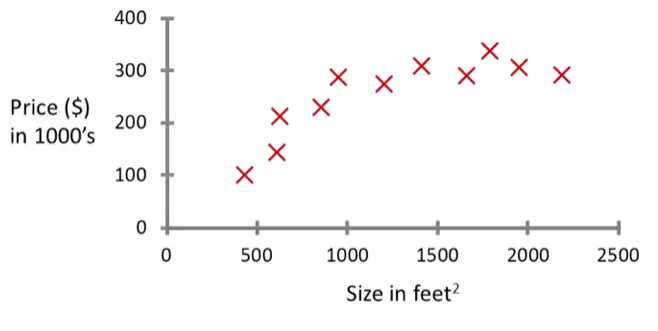
\includegraphics{img/sl1.png}

Here on the horizontal axis, the size of different houses in square
feet, and on the vertical axis, the price of different houses in
thousands of dollars.

So. Given this data, let's say we own a house that is, say 750 square
feet and hoping to sell the house and we want to know how much we can
get for the house.

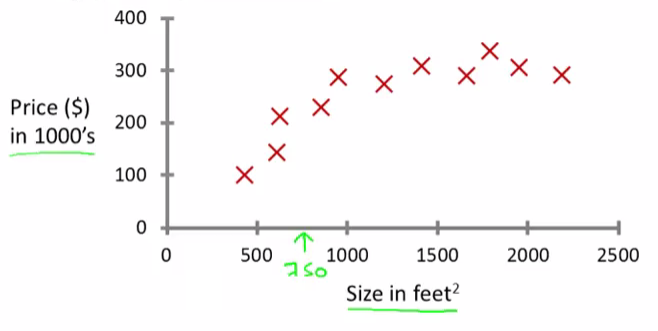
\includegraphics{img/sl2.png}

So how can the learning algorithm help?

One thing a learning algorithm might be able to do is put a straight
line through the data or to \textbf{``fit''} a straight line to the data
and, based on that, it looks like maybe the house can be sold for maybe
about \$150,000.

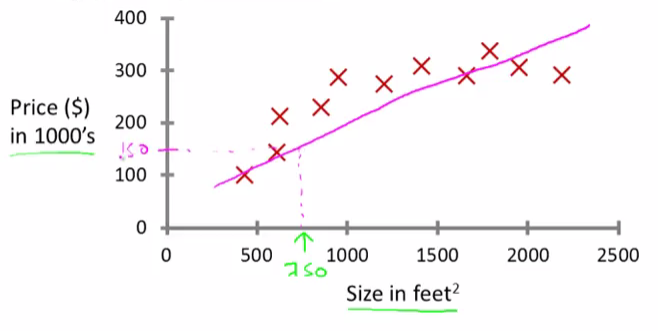
\includegraphics{img/sl3.png}

But maybe this isn't the only learning algorithm we can use. There might
be a better one. For example, instead of sending a straight line to the
data, we might decide that it's better to fit a \emph{quadratic
function} or a \emph{second-order polynomial} to this data.

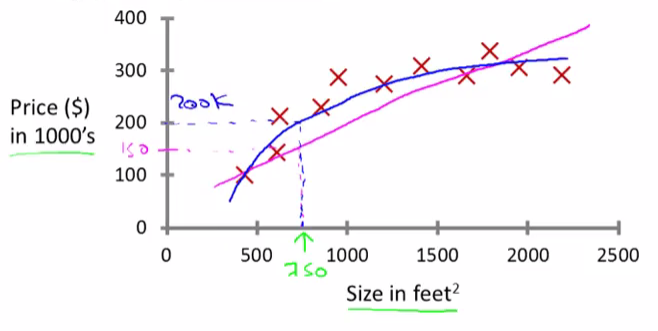
\includegraphics{img/sl4.png}

If we do that, and make a prediction here, then it looks like, well,
maybe we can sell the house for closer to \$200,000.

This is an example of a supervised learning algorithm.

The term supervised learning refers to the fact that we gave the
algorithm a data set in which the \textbf{``right answers''} were given.

The example above is also called a regression problem. A regression
problem is when we try to predict a \textbf{continuous} value output.
Namely the price in the example.

Here's another supervised learning example. Let's say we want to look at
medical records and try to predict of a breast cancer as malignant or
benign. If someone discovers a breast tumor, a lump in their breast, a
malignant tumor is a tumor that is harmful and dangerous and a benign
tumor is a tumor that is harmless. Let's see a collected data set and
suppose in the data set we have the size of the tumor on the horizontal
axis and on the vertical axis we plot one or zero, yes or no, whether or
not these are examples of tumors we've seen before are malignant (which
is one) or zero if not malignant or benign.

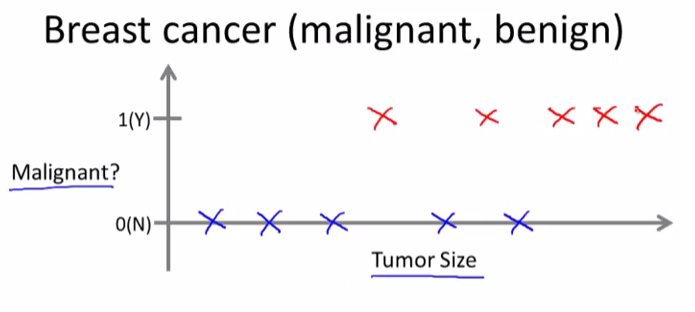
\includegraphics{img/sl5.png}

In this data set we have five examples of benign tumors, and five
examples of malignant tumors.

Let's say a person who tragically has a breast tumor, and let's say her
breast tumor size is known (rose arrow in the following figure).

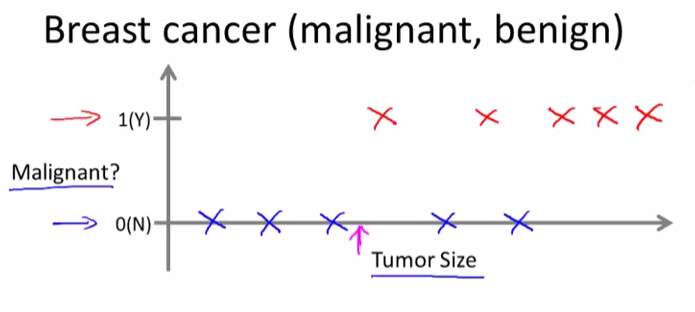
\includegraphics{img/sl6.png}

The machine learning question is, can you estimate what is the
probability that a tumor is malignant versus benign? To introduce a bit
more terminology this is an example of a \textbf{\emph{classification}}
problem.

The term classification refers to the fact that here we're trying to
predict a \textbf{discrete} value output: zero or one, malignant or
benign. And it turns out that in classification problems sometimes you
can have more than two values for the two possible values for the
output.

In classification problems there is another way to plot this data. Let's
use a slightly different set of symbols to plot this data. So if tumor
size is going to be the attribute that we are going to use to predict
malignancy or benignness, we can also draw the data like this.

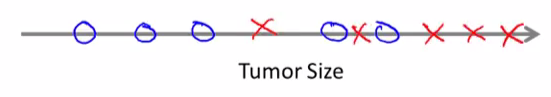
\includegraphics{img/sl7.png}

All we did was we took the data set on top and just mapped it down using
different symbols. So instead of drawing crosses, we are now going to
draw \texttt{O}'s for the benign tumors.

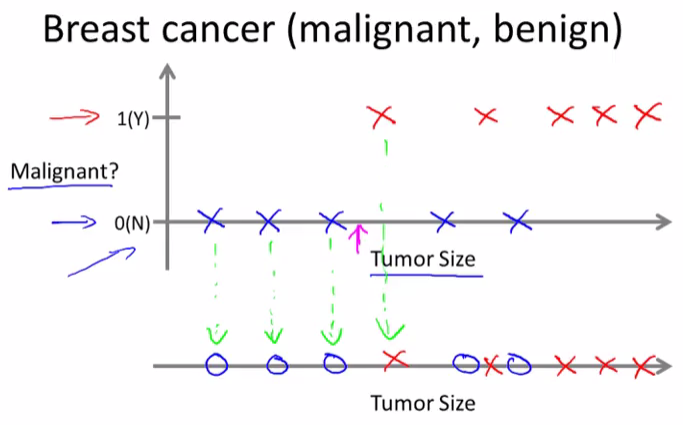
\includegraphics{img/sl8.png}

Now, in this example we use only one \textbf{feature} or one attribute,
mainly, the \emph{tumor size} in order to predict whether the tumor is
malignant or benign.

In other machine learning problems we may have more than one feature.

Here's an example. Let's say that instead of just knowing the tumor
size, we know both the age of the patients and the tumor size. In that
case maybe the data set will look like this.

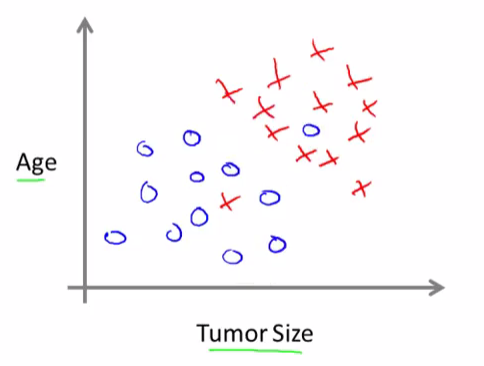
\includegraphics{img/sl9.png}

So, let's say a person who tragically has a tumor. And maybe, their
tumor size and age falls around there (rose point):

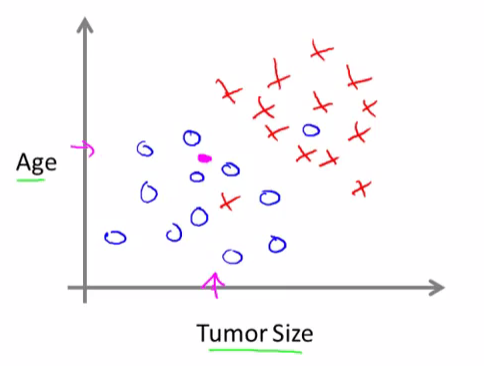
\includegraphics{img/sl10.png}

So given a data set like this, what the learning algorithm might do is
throw a straight line through the data to try to separate out the
malignant tumors from the benign ones. And with this, hopefully we can
decide that the person's tumor falls on this benign side and is
therefore more likely to be benign than malignant.

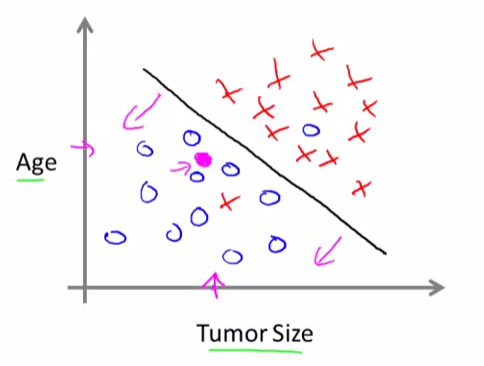
\includegraphics{img/sl11.png}

In this example we had \textbf{two features}, namely, the age of the
patient and the size of the tumor. In other machine learning problems we
will often have more features.

Most interesting learning algorithms is a learning algorithm that can
deal with, not just two or three or five features, but an
\textbf{infinite number of features}. So how do you deal with an
infinite number of features. How do you even store an infinite number of
things on the computer when your computer is gonna run out of memory.

\section*{Unsupervised Learning}\label{unsupervised-learning}
\addcontentsline{toc}{section}{Unsupervised Learning}

The second major type of machine learning problem is called Unsupervised
Learning.

The difference between Unsupervised Learning and Supervised Learning is
that in Supervised Learning we are told explicitly what is the so-called
right answers (data are labeled).

In Unsupervised Learning, we're given data that doesn't have any labels
or that all has the same label or really no labels. Like in this
example:

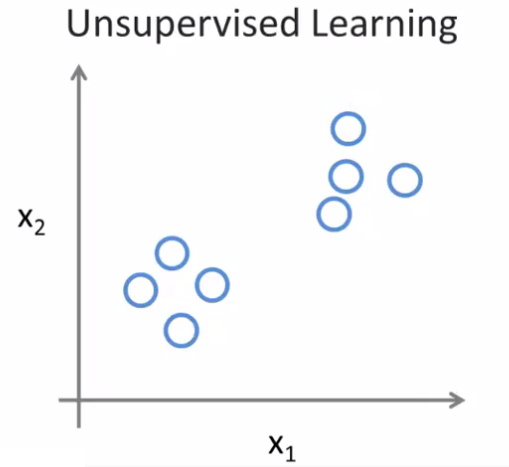
\includegraphics{img/ul1.png}

So we're given the data set and we're not told what to do with it and
we're not told what each data point is. Instead we're just told, here is
a data set. Can you find some structure in the data?

Given this data set, an Unsupervised Learning algorithm might decide
that the data lives in two different clusters.

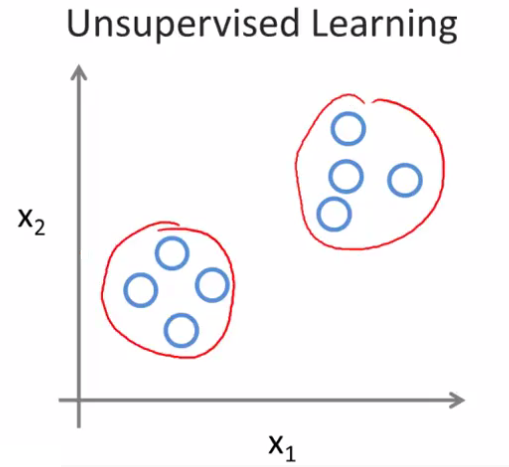
\includegraphics{img/ul2.png}

This is called a \textbf{clustering} algorithm.

Here are two examples where Unsupervised Learning or clustering is used.

Social network analysis:

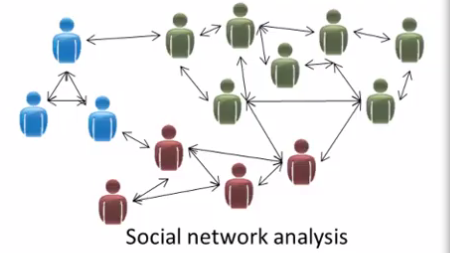
\includegraphics{img/ul3.png}

So given knowledge about which friends you email the most or given your
Facebook friends or your Google+ circles, can we automatically identify
which are cohesive groups of friends, also which are groups of people
that all know each other?

Market segmentation:

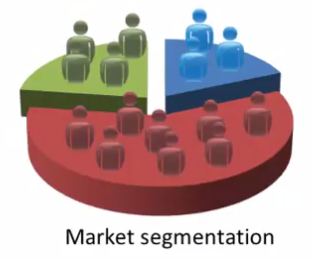
\includegraphics{img/ul4.png}

Many companies have huge databases of customer information. So, can you
look at this customer data set and automatically discover market
segments and automatically group your customers into different market
segments so that you can automatically and more efficiently sell or
market your different market segments together?

This is Unsupervised Learning because we have all this customer data,
but we don't know in advance what are the market segments and for the
customers in our data set, we don't know in advance who is in market
segment one, who is in market segment two, and so on. But we have to let
the algorithm discover all this just from the data.

◼

\part{Supervised Learning}\label{part-supervised-learning}
\addcontentsline{toc}{chapter}{(PART) Supervised Learning}

\part{Regression}\label{part-regression}
\addcontentsline{toc}{chapter}{(PART) Regression}

\chapter{Linear Regression}\label{linear-regression}

\section{Notation}\label{notation}

In general, we will let \(x_{ij}\) represent the value of the \(j\)th
variable for the \(i\)th observation, where \(i=1,2,\ldots,n\) and
\(j=1,2,\ldots,p\). We will use \(i\) to index the samples or
observations (from \(1\) tp \(n\)) and \(j\) will be used to index the
variables (or features) (from \(1\) to \(p\)). We let \(\textbf{X}\)
denote a \(n \times p\) matrix whose \((i,j)\)th element is \(x_{ij}\).
That is,

\[ \textbf{X}  = \begin{pmatrix}
    x_{11} & x_{12} & x_{13} & \dots  & x_{1p} \\
    x_{21} & x_{22} & x_{23} & \dots  & x_{2p} \\
    \vdots & \vdots & \vdots & \ddots & \vdots \\
    x_{n1} & x_{n2} & x_{n3} & \dots  & x_{np}
\end{pmatrix} \]

Note that it is useful to visualize \(\textbf{X}\) as a spreadsheet of
numbers with \(n\) rows and \(p\) columns. We will write the rows of
\(\textbf{X}\) as \(x_1 , x_2 , \ldots, x_n\). Here \(x_i\) is a vector
of length \(p\), containing the \(p\) variable measurements for the
\(i\)th observation. That is,

\[ x_i = \begin{pmatrix}
    x_{i1} \\
    x_{i2} \\
    \vdots \\
    x_{ip}
\end{pmatrix}\]

(Vectors are by default represented as columns.)

We will write the columns of \(\textbf{X}\) as
\(\textbf{x}_1 , \textbf{x}_2, \ldots, \textbf{x}_p\). Each is a vector
of length \(n\). That is,

\[ \textbf{x}_j = \begin{pmatrix}
    \textbf{x}_{1j} \\
    \textbf{x}_{2j} \\
    \vdots \\
    \textbf{x}_{nj}
\end{pmatrix}\]

Using this notation, the matrix \(\textbf{X}\) can be written as

\[ \textbf{X} = (\textbf{x}_1  \textbf{x}_2 \ldots \textbf{x}_p) \]

or

\[ \textbf{X} = \begin{pmatrix}
    x_{1}^T \\
    x_{2}^T \\
    \vdots \\
    x_{n}^T
\end{pmatrix}\]

The \(^T\) notation denotes the transpose of a matrix or vector.

We use \(y_i\) to denote the \(i\)th observation of the variable on
which we wish to make predictions. We write the set of all \(n\)
observations in vector form as

\[ \textbf{y} = \begin{pmatrix}
    y_{1}^T \\
    y_{2}^T \\
    \vdots \\
    y_{n}^T
\end{pmatrix}\]

Then the observed data consists of
\(\{(x_1, y_1), (x_2 , y_2 ), \ldots , (x_n , y_n )\}\), where each
\(x_i\) is a vector of length \(p\). (If \(p = 1\), then \(x_i\) is
simply a scalar).

\section{Model Representation}\label{model-representation}

Let's consider the example about predicting housing prices. We're going
to use this data set as an example,

\begin{figure}[htbp]
\centering
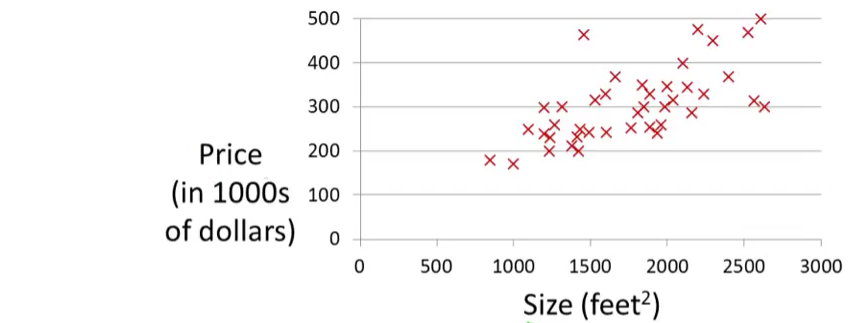
\includegraphics{img/mr1.png}
\caption{}
\end{figure}

Suppose that there is a person trying to sell a house of size 1250
square feet and he wants to know how much he might be able to sell the
house for. One thing we could do is fit a model. Maybe fit a straight
line to this data. Looks something like this,

\begin{figure}[htbp]
\centering
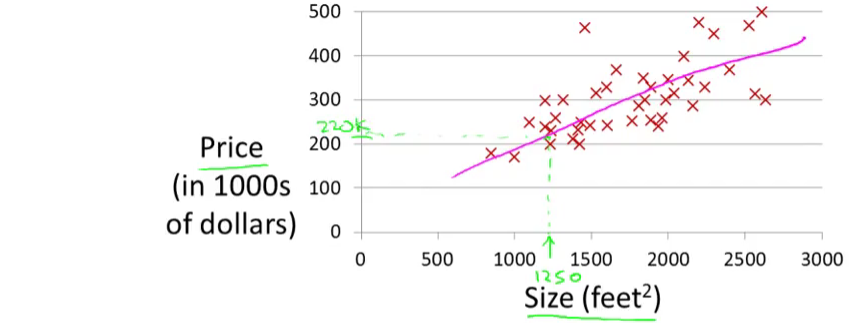
\includegraphics{img/mr2.png}
\caption{}
\end{figure}

and based on that, maybe he can sell the house for around \$220,000.
Recall that this is an example of a supervised learning algorithm. And
it's supervised learning because we're given the ``right answer'' for
each of our examples. More precisely, this is an example of a regression
problem where the term regression refers to the fact that we are
predicting a real-valued output namely the price.

More formally, in supervised learning, we have a data set and this data
set is called a \textbf{training set}. So for housing prices example, we
have a training set of different housing prices and our job is to learn
from this data how to predict prices of the houses.

Let's define some notation from this data set:

\begin{itemize}
\tightlist
\item
  The size of the house is the input variable.
\item
  The house price is the output variable.
\item
  The input variables are typically denoted using the variable symbol
  \(X\),
\item
  The inputs go by different names, such as \emph{predictors},
  \emph{independent variables}, \emph{features}, \emph{predictor} or
  sometimes just \emph{variables}.
\item
  The output variable is often called the \emph{response},
  \emph{dependent variable} or \emph{target}, and is typically denoted
  using the symbol \(Y\).
\item
  \((x_i,y_i)\) is the \(i\)th training example.
\item
  The set of \(\{(x_i, y_i)\}\) is the training set.
\item
  \(n\) is the number of training examples.
\end{itemize}

So here's how this supervised learning algorithm works. Suppose that we
observe a quantitative response \(Y\) and \(p\) different predictors,
\(X_1 , X_2 ,\ldots, X_p\) . We assume that there is some relationship
between \(Y\) and \(X = (X_1 , X_2 ,\ldots, X_p)\), which can be written
in the very general form

\[Y = f(X) + \epsilon\]

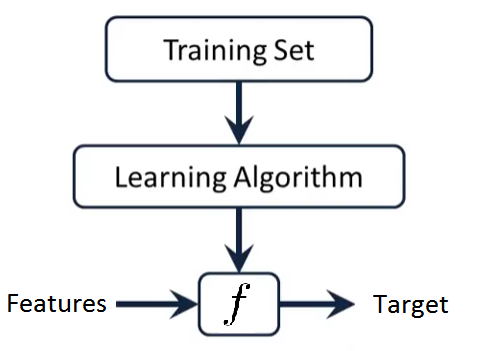
\includegraphics{img/mr3.png}

Here \(f\) is some fixed but unknown function of
\(X_1 , X_2 ,\ldots, X_p\) , and \(\epsilon\) is a random error term,
which is independent of \(X\) and has mean zero. The \(f\) function is
also called \emph{hypothesis} in Machine Learning. In general, the
function \(f\) may involve more than one input variable. In essence,
Supervised Learning refers to a set of approaches for estimating \(f\).

\section{\texorpdfstring{Why Estimate \(f\)
?}{Why Estimate f ?}}\label{why-estimate-f}

There are two main reasons that we may wish to estimate \(f\):
\emph{prediction} and \emph{inference}.

\subsection*{Prediction}\label{prediction}
\addcontentsline{toc}{subsection}{Prediction}

In many situations, a set of inputs \(X\) are readily available, but the
output \(Y\) cannot be easily obtained. In this setting, since the error
term averages to zero, we can predict \(Y\) using

\[ \hat{Y} = \hat{f}(X) \]

where \(\hat{f}\) represents our estimate for \(f\), and \(\hat{Y}\)
represents the resulting prediction for \(Y\). Like in the example above
about predicting housing prices.

We can measure the accuracy of \(\hat{Y}\) by using a \textbf{cost
function}. In the regression models, the most commonly-used measure is
the \emph{mean squared error} (MSE), given by

\[ MSE = \frac{1}{n} \sum_{i=1}^{n} (y_i - \hat{f}(x_i))^2\]

\subsection*{Inference}\label{inference}
\addcontentsline{toc}{subsection}{Inference}

We are often interested in understanding the way that \(Y\) is affected
as \(X_1 , X_2 ,\ldots, X_p\) change. In this situation we wish to
estimate \(f\) , but our goal is not necessarily to make predictions for
\(Y\). We instead want to understand the relationship between \(X\) and
\(Y\), or more specifically, to understand how \(Y\) changes as a
function of \(X_1 , X_2 ,\ldots, X_p\). In this case, one may be
interested in answering the following questions:

\begin{itemize}
\tightlist
\item
  Which predictors are associated with the response?
\item
  What is the relationship between the response and each predictor?
\item
  Can the relationship between Y and each predictor be adequately
  summarized using a linear equation, or is the relationship more
  complicated?
\end{itemize}

\section{Simple Linear Regression
Model}\label{simple-linear-regression-model}

\emph{Simple linear regression} is a very straightforward approach for
predicting a quantitative response \(Y\) on the basis of a single
predictor variable \(X\). It assumes that there is approximately a
linear relationship between \(X\) and \(Y\). Mathematically, we can
write this linear relationship as

\[ Y = \beta_0 + \beta_1 X + \epsilon \]
\[Y \approx \beta_0 + \beta_1 X\]

where \(\beta_0\) and \(\beta_1\) are two unknown constants that
represent the \emph{intercept} and \emph{slope}, also known as
\textbf{\emph{coefficients}} or \emph{parameters}, and \(\epsilon\) is
the error term.

Given some estimates \(\hat{\beta_0}\) and \(\hat{\beta_1}\) for the
model coefficients, we predict future inputs \(x\) using

\[\hat{y} = \hat{\beta_0} + \hat{\beta_1} x\]

where \(\hat{y}\) indicates a prediction of \(Y\) on the basis of
\(X = x\). The \emph{hat} symbol, \(\hat{}\), denotes an estimated
value.

\section{Estimating the Coefficients}\label{estimating-the-coefficients}

Let \(\hat{y}_i = \hat{\beta_0} + \hat{\beta_1} x_i\) be the prediction
for \(Y\) based on the \(i\)th value of \(X\). Then
\(e_i = y_i - \hat{y}_i\) represents the \(i\)th
\textbf{\emph{residual}}.

We define the \textbf{\emph{residual sum of squares}} (\textbf{RSS}) as

\[  \begin{aligned}
RSS &= e_1^2 + e_2^2 + \ldots + e_n^2 \\
    &= \sum_{i=1}^{n} e_i^2
 \end{aligned}  \]

or equivantly as

\[ \begin{aligned}
RSS &= (y_1 - \hat{\beta_0} - \hat{\beta_1} x_1)^2 + (y_2 - \hat{\beta_0} - \hat{\beta_1} x_2)^2 + \ldots + (y_n - \hat{\beta_0} - \hat{\beta_1} x_n)^2 \\
    &= \sum_{i=1}^{n} (y_i - \hat{\beta_0} - \hat{\beta_1} x_i)^2
\end{aligned} \]

The \emph{least squares} approach chooses \(\hat{\beta_0}\) and
\(\hat{\beta_1}\) to minimize the RSS. The minimizing values can be show
to be

\[  \begin{aligned}
\hat{\beta_1} &=  \frac{\sum_{i=1}^{n} (x_i - \bar{x})(y_i - \bar{y})  }{\sum_{i=1}^{n} (x_i - \bar{x})^2 } = \frac{s_{xy}}{s_x^2} \\
\text{and} \\
\hat{\beta_0} &= \bar{y} - \hat{\beta_1} \bar{x}
\end{aligned}  \]

where:

\begin{itemize}
\tightlist
\item
  \(\bar{x}=\frac{1}{n}\sum_{i=1}^nx_i\) is the \emph{sample mean}.
\item
  \(s_x^2=\frac{1}{n}\sum_{i=1}^n(x_i-\bar{x})^2\) is the \emph{sample
  variance}. The sample standard deviation is \(s_x=\sqrt{s_x^2}\).
\item
  \(s_{xy}=\frac{1}{n}\sum_{i=1}^n(x_i-\bar{x})(y_i-\bar{y})\) is the
  \emph{sample covariance}. It measures the degree of linear association
  between \(x_1,\ldots,x_n\) and \(y_1,\ldots,y_n\). Once scaled by
  \(s_xs_y\), it gives the \emph{sample correlation coefficient},
  \(r_{xy}=\frac{s_{xy}}{s_xs_y}\).
\end{itemize}

\begin{rmdinsight}
Click here to see the influence of the distance employed in the sum of
squares. Try to minimize the sum of squares for the different datasets.
The choices of intercept and slope that minimize the sum of squared
distances for a kind of distance are not the optimal for a different
kind of distance.
\end{rmdinsight}

\section{Assessing the Accuracy of the Coefficient
Estimates}\label{assessing-the-accuracy-of-the-coefficient-estimates}

The standard error of an estimator reflects how it varies under repeated
sampling. We have

\[ \text{SE}(\hat{\beta_1})^2 =  \frac{\sigma^2}{\sum_{i=1}^{n} (x_i - \bar{x})^2} \]

\[ \text{SE}(\hat{\beta_0})^2 = \sigma^2 \bigg[ \frac{1}{n} +  \frac{\bar{x}^2}{\sum_{i=1}^{n} (x_i - \bar{x})^2} \bigg] \]

where \(\sigma^2 = Var(\epsilon)\)

In general, \(\sigma^2\) is know known, but can be estimated from the
data. The estimate of \(\sigma\) is known as the \emph{residual standard
error}, and is given by

\[ \text{RSE} = \sqrt{\frac{\text{RSS}}{(n-2)}} \]

These standard errors can be used to compute \emph{confidence
intervals}. A \(95\%\) confidence interval is defined as a range of
values such that with \(95\%\) probability, the range will contain the
true unknown value of the parameter. It has the form

\[ \hat{\beta_1} \pm 2 \cdot \text{SE}(\hat{\beta_1}) \]

That is, there is approximately a \(95\%\) chance that the interval

\[ \bigg[  \hat{\beta_1} - 2 \cdot \text{SE}(\hat{\beta_1}), \hat{\beta_1} + 2 \cdot \text{SE}(\hat{\beta_1})   \bigg] \]

will contain the true value of \(\beta_1\). Similarly, a confidence
interval for \(\beta_0\) approximately takes the form

\[ \hat{\beta_0} \pm 2 \cdot \text{SE}(\hat{\beta_0}) \]

\subsection*{Hypothesis testing}\label{hypothesis-testing}
\addcontentsline{toc}{subsection}{Hypothesis testing}

Standard errors can also be used to perform \emph{hypothesis tests} on
the coefficients. The most common hypothesis test involves testing the
\emph{null hypothesis} of

\[ H_0 : \text{There is no relationship between} \, X \, \text{and} \, Y \]

versus the \emph{alternative hypothesis}

\[ H_1 : \text{There is some relationship between} \, X \, \text{and} \, Y \]

Mathematically, this corresponds to testing

\[ H_0 : \beta_1 = 0 \]

versus

\[ H_1 : \beta_1 \neq 0 \]

since if \(\beta_1 = 0\) then the simple linear regression model reduces
to \(Y = \beta_0 + \epsilon\), and \(X\) is not associated with \(Y\).

To test the null hypothesis \(H_0\), we compute a
\textbf{\emph{t-statistic}}, given by

\[ t = \frac{\hat{\beta_1} - 0}{\text{SE}(\hat{\beta_1})} \]

This will have a \(t\)-distribution (\emph{Student}) with \(n-2\)
degrees of freedom, assuming \(\beta_1=0\).

Using statistical software, it is easy to compute the probability of
observing any value equal to \(|t|\) or larger. We call this probability
the \textbf{\emph{p-value}}.

If p-value is small enough (typically under \(0.01\) (\(1\%\) error) or
\(0.05\) (\(5\%\) error)) we reject the null hypothesis, that is we
declare a relationship to exist between \(X\) and \(Y\).

\section{ANOVA and model fit}\label{anova-and-model-fit}

\subsection{ANOVA}\label{anova}

In this section we will see how the variance of \(Y\) is decomposed into
two parts, each one corresponding to the regression and to the error,
respectively. This decomposition is called the \emph{ANalysis Of
VAriance} (ANOVA).

Before explaining ANOVA, it is important to recall an interesting
result: \emph{the mean of the fitted values \(\hat Y_1,\ldots,\hat Y_n\)
is the mean of \(Y_1,\ldots, Y_n\)}. This is easily seen if we plug-in
the expression of \(\hat\beta_0\):

\begin{align*}
\frac{1}{n}\sum_{i=1}^n \hat Y_i=\frac{1}{n}\sum_{i=1}^n \left(\hat \beta_0+\hat\beta_1X_i\right)=\hat \beta_0+\hat\beta_1\bar X=\left(\bar Y - \hat\beta_1\bar X \right) + \hat\beta_1\bar X=\bar Y.
\end{align*}

The ANOVA decomposition considers the following measures of variation
related with the response:

\begin{itemize}
\tightlist
\item
  \(\text{SST}=\sum_{i=1}^n\left(Y_i-\bar Y\right)^2\), the
  \textbf{total sum of squares}. This is the \emph{total variation} of
  \(Y_1,\ldots,Y_n\), since \(\text{SST}=ns_y^2\), where \(s_y^2\) is
  the sample variance of \(Y_1,\ldots,Y_n\).
\item
  \(\text{SSR}=\sum_{i=1}^n\left(\hat Y_i-\bar Y\right)^2\), the
  \textbf{regression sum of squares}\footnote{Recall that SSR is
    different from RSS (Residual Sum of Squares}. This is the variation
  explained by the regression line, that is, \emph{the variation from
  \(\bar Y\) that is explained by the estimated conditional mean
  \(\hat Y_i=\hat\beta_0+\hat\beta_1X_i\)}.
  \(\text{SSR}=ns_{\hat y}^2\), where \(s_{\hat y}^2\) is the sample
  variance of \(\hat Y_1,\ldots,\hat Y_n\).
\item
  \(\text{SSE}=\sum_{i=1}^n\left(Y_i-\hat Y_i\right)^2\), the
  \textbf{sum of squared errors}\footnote{Recall that SSE and RSS (for
    \((\hat \beta_0,\hat \beta_1)\)) are just different names for
    referring to the same quantity:
    \(\text{SSE}=\sum_{i=1}^n\left(Y_i-\hat Y_i\right)^2=\sum_{i=1}^n\left(Y_i-\hat \beta_0-\hat \beta_1X_i\right)^2=\mathrm{RSS}\left(\hat \beta_0,\hat \beta_1\right)\).}.
  Is the variation around the conditional mean. Recall that
  \(\text{SSE}=\sum_{i=1}^n \hat\varepsilon_i^2=(n-2)\hat\sigma^2\),
  where \(\hat\sigma^2\) is the sample variance of
  \(\hat \varepsilon_1,\ldots,\hat \varepsilon_n\).
\end{itemize}

The ANOVA decomposition is

\begin{align*}
\underbrace{\text{SST}}_{\text{Variation of }Y_i's} = \underbrace{\text{SSR}}_{\text{Variation of }\hat Y_i's} + \underbrace{\text{SSE}}_{\text{Variation of }\hat \varepsilon_i's}
\end{align*}

The graphical interpretation of this equation is shown in the following
figures.

\begin{figure}

{\centering 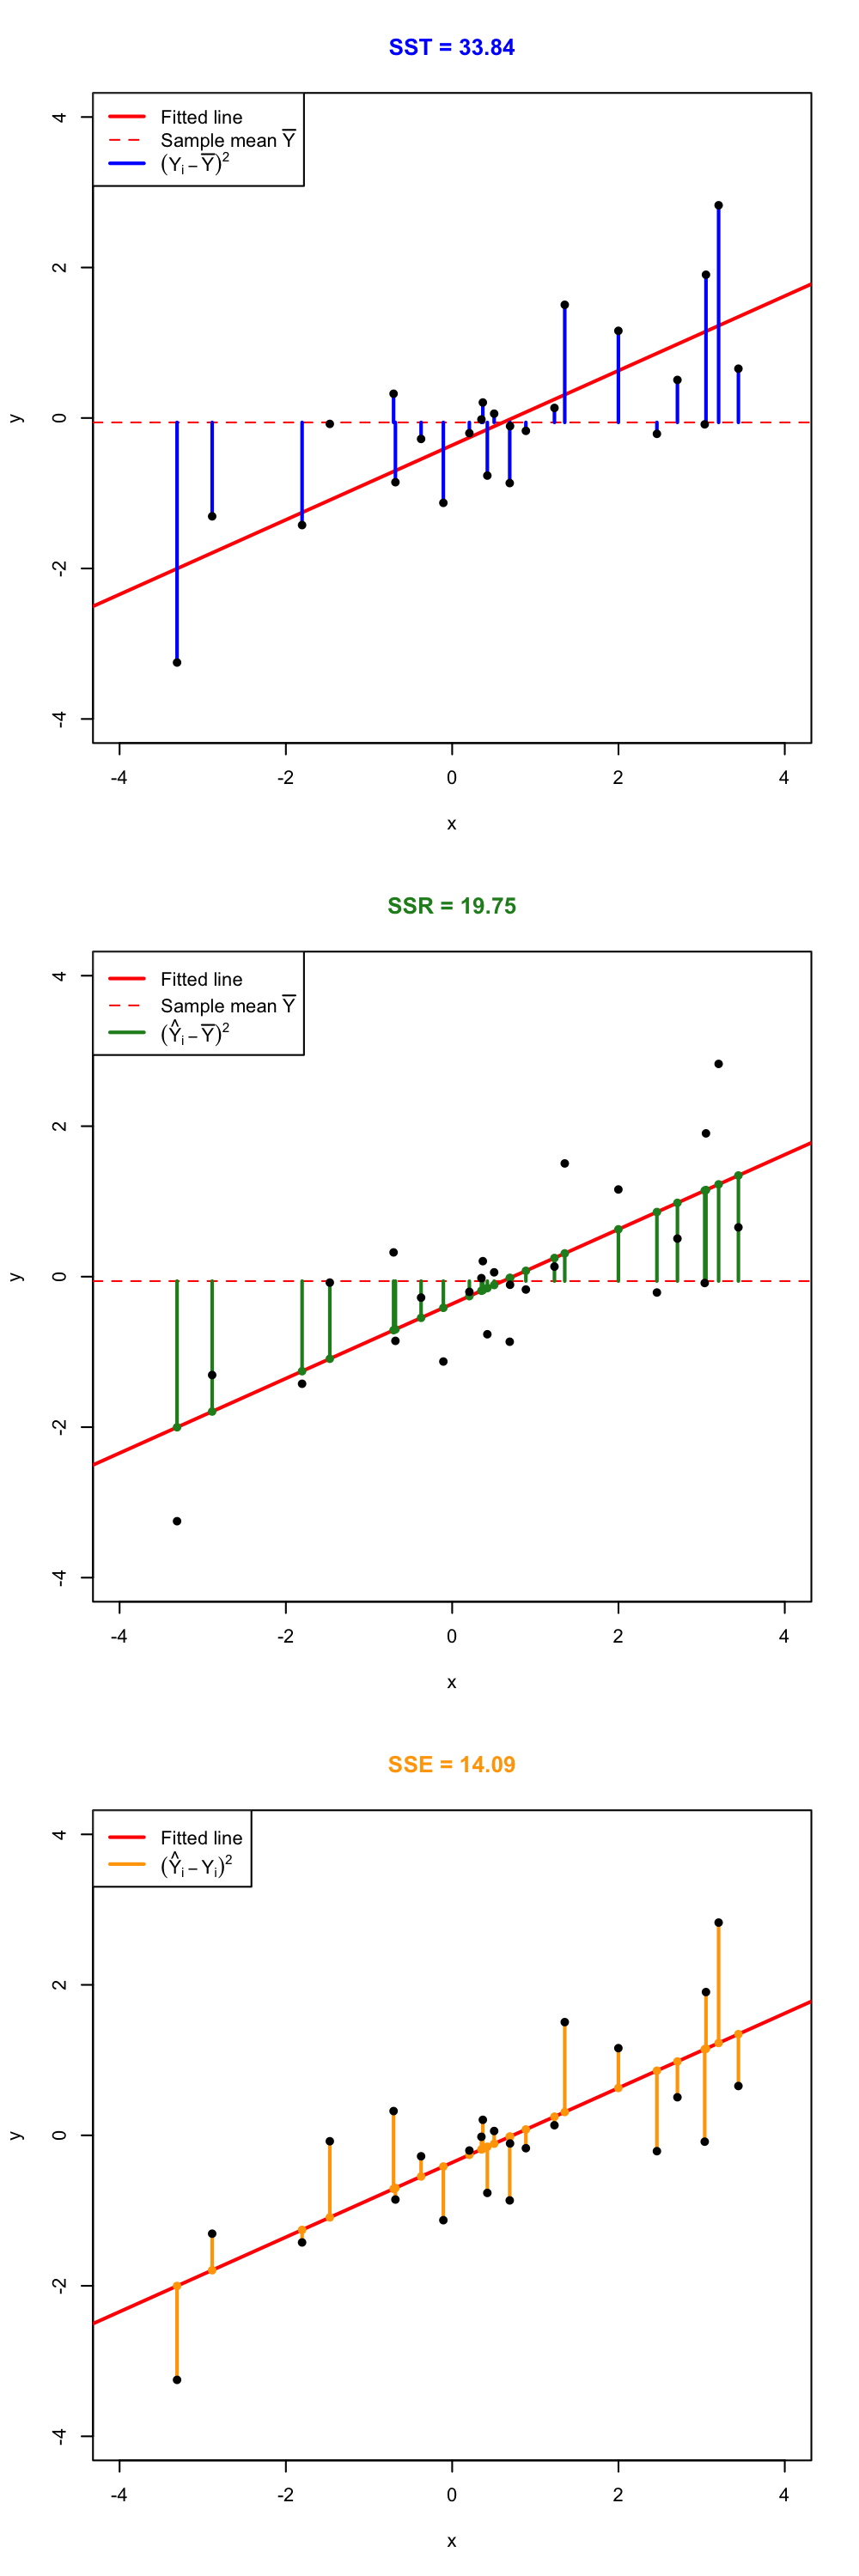
\includegraphics[width=0.7\linewidth]{img/anova} 

}

\caption{Visualization of the ANOVA decomposition. SST measures the variation of $Y_1,\ldots,Y_n$ with respect to $\bar Y$. SST measures the variation with respect to the conditional means, $\hat \beta_0+\hat\beta_1X_i$. SSE collects the variation of the residuals.}\label{fig:anova}
\end{figure}

\begin{rmdinsight}
Click here to see the ANOVA decomposition and its dependence on
\(\sigma^2\) and \(\hat\sigma^2\).'
\end{rmdinsight}

The ANOVA table summarizes the decomposition of the variance. Here is
given in the layout employed by \texttt{R}.

\begin{longtable}[]{@{}llllll@{}}
\toprule
& Degrees of freedom & Sum Squares & Mean Squares & \(F\)-value &
\(p\)-value\tabularnewline
\midrule
\endhead
Predictor & \(1\) & SSR & \(\frac{\text{SSR}}{1}\) &
\(\frac{\text{SSR}/1}{\text{SSE}/(n-2)}\) & \(p\)\tabularnewline
Residuals & \(n - 2\) & SSE & \(\frac{\text{SSE}}{n-2}\) &
&\tabularnewline
\bottomrule
\end{longtable}

The \texttt{anova} function in \texttt{R} takes a model as an input and
returns the ANOVA table.

The ``\(F\)-value'' of the ANOVA table represents the value of the
\(F\)-statistic \(\frac{\text{SSR}/1}{\text{SSE}/(n-2)}\). This
statistic is employed to test

\begin{align*}
H_0:\beta_1=0\quad\text{vs.}\quad H_1:\beta_1\neq 0,
\end{align*}

that is, the hypothesis of no linear dependence of \(Y\) on \(X\). The
result of this test is completely equivalent to the \(t\)-test for
\(\beta_1\) that we saw previously in the Hypothesis testing (this is
something \emph{specific for simple linear regression} -- the \(F\)-test
will not be equivalent to the \(t\)-test for \(\beta_1\) in the Mulitple
Linear Regression).

It happens that

\begin{align*}
F=\frac{\text{SSR}/1}{\text{SSE}/(n-2)}\stackrel{H_0}{\sim} F_{1,n-2},
\end{align*}

where \(F_{1,n-2}\) is the \emph{Snedecor's \(F\)
distribution}\footnote{The \(F_{n,m}\) distribution arises as the
  quotient of two independent random variables \(\chi^2_n\) and
  \(\chi^2_m\), \(\frac{\chi^2_n/n}{\chi^2_m/m}\).} with \(1\) and
\(n-2\) degrees of freedom.

If \(H_0\) is true, then \(F\) is expected to be \emph{small} since SSR
will be close to zero. The \(p\)-value of this test is the same as the
\(p\)-value of the \(t\)-test for \(H_0:\beta_1=0\).

\subsection{\texorpdfstring{The \(R^2\)
Statistic}{The R\^{}2 Statistic}}\label{the-r2-statistic}

To calculate \(R^2\), we use the formula

\[ R^2 = \frac{\text{TSS} - \text{RSS}}{\text{TSS}} = 1- \frac{\text{RSS}}{\text{TSS}} \]

where \(\text{TSS} = \sum (y_i - \bar{y})^2\) is the \emph{total sum of
squared}.

\(R^2\) measures the \emph{proportion of variability in} \(Y\)
\emph{that can be explained using} \(X\). An \(R^2\) statistic that is
close to 1 indicates that a large proportion of the variability in the
response has been explained by the regression. A number near 0 indicates
that the regression did not explain much of the variability in the
response; this might occur because the linear model is wrong, or the
inherent error \(\sigma^2\) is high, or both.

It can be shown that in this simple linear linear regression setting
that \(R^2 = r^2\), where \(r\) is the correlation between \(X\) and
\(Y\):

\[ r = \frac{cov(X,Y)}{\sigma_X \sigma_Y} \]

\begin{rmdcaution}
\(R^2\) does not measure the correctness of a linear model but its
\textbf{usefulness} (for prediction, for \emph{explaining the variance}
of \(Y\)), assuming the model is correct.

Trusting blindly the \(R^2\) can lead to catastrophic conclusions, since
the model may not be correct.
\end{rmdcaution}

So remember:

\begin{rmdinsight}
A large \(R^2\) means \emph{nothing} if the \textbf{assumptions of the
model do not hold}. \(R^2\) is the proportion of variance of \(Y\)
explained by \(X\), but, of course, \emph{only when the linear model is
correct}.
\end{rmdinsight}

◼

\chapter*{PW 1}\label{pw-1}
\addcontentsline{toc}{chapter}{PW 1}

\section{\texorpdfstring{Some \texttt{R}
basics}{Some R basics}}\label{some-r-basics}

\subsection{Basic Commands}\label{basic-commands}

\texttt{R} uses functions to perform operations. To run a function
called \texttt{funcname},we type \texttt{funcname(input1,\ input2)} ,
where the inputs (or arguments) \texttt{input1} and \texttt{input2} tell
\texttt{R} how to run the function. A function can have any number of
inputs. For example, to create a vector of numbers, we use the function
\texttt{c()} (for \emph{concatenate}).

\begin{Shaded}
\begin{Highlighting}[]
\NormalTok{x <-}\StringTok{ }\KeywordTok{c}\NormalTok{(}\DecValTok{1}\NormalTok{,}\DecValTok{3}\NormalTok{,}\DecValTok{2}\NormalTok{,}\DecValTok{5}\NormalTok{)}
\NormalTok{x}
\CommentTok{#ans> [1] 1 3 2 5}
\end{Highlighting}
\end{Shaded}

Note that the \texttt{\textgreater{}} is not part of the command;
rather, it is printed by \texttt{R} to indicate that it is ready for
another command to be entered. We can also save things using \texttt{=}
rather than \texttt{\textless{}-}. Note that the answer in the code
above is followed by \texttt{\#ans\textgreater{}} while in the
\texttt{R} console it is not.

\begin{Shaded}
\begin{Highlighting}[]
\NormalTok{x =}\StringTok{ }\KeywordTok{c}\NormalTok{(}\DecValTok{1}\NormalTok{,}\DecValTok{6}\NormalTok{,}\DecValTok{2}\NormalTok{)}
\NormalTok{x}
\CommentTok{#ans> [1] 1 6 2}
\NormalTok{y =}\StringTok{ }\KeywordTok{c}\NormalTok{(}\DecValTok{1}\NormalTok{,}\DecValTok{4}\NormalTok{,}\DecValTok{3}\NormalTok{)}
\KeywordTok{length}\NormalTok{(x)}
\CommentTok{#ans> [1] 3}
\KeywordTok{length}\NormalTok{(y)}
\CommentTok{#ans> [1] 3}
\NormalTok{x+y}
\CommentTok{#ans> [1]  2 10  5}
\end{Highlighting}
\end{Shaded}

Hitting the \emph{up arrow} multiple times will display the previous
commands, which can then be edited. This is useful since one often
wishes to repeat a similar command.

The \texttt{ls()} function allows us to look at a list of all of the
objects, such \texttt{ls()} as data and functions, that we have saved so
far. The \texttt{rm()} function can be used to delete any object that we
don't want.

\begin{Shaded}
\begin{Highlighting}[]
\KeywordTok{ls}\NormalTok{()}
\CommentTok{#ans> [1] "x" "y"}
\KeywordTok{rm}\NormalTok{(x)}
\KeywordTok{ls}\NormalTok{()}
\CommentTok{#ans> [1] "y"}
\end{Highlighting}
\end{Shaded}

\subsection{Vectors}\label{vectors}

\begin{Shaded}
\begin{Highlighting}[]

\CommentTok{# A handy way of creating sequences is the operator :}
\CommentTok{# Sequence from 1 to 5}
\DecValTok{1}\NormalTok{:}\DecValTok{5}
\CommentTok{#ans> [1] 1 2 3 4 5}

\CommentTok{# Storing some vectors}
\NormalTok{vec <-}\StringTok{ }\KeywordTok{c}\NormalTok{(-}\FloatTok{4.12}\NormalTok{, }\DecValTok{0}\NormalTok{, }\FloatTok{1.1}\NormalTok{, }\DecValTok{1}\NormalTok{, }\DecValTok{3}\NormalTok{, }\DecValTok{4}\NormalTok{)}
\NormalTok{vec}
\CommentTok{#ans> [1] -4.12  0.00  1.10  1.00  3.00  4.00}

\CommentTok{# Entry-wise operations}
\NormalTok{vec +}\StringTok{ }\DecValTok{1}
\CommentTok{#ans> [1] -3.12  1.00  2.10  2.00  4.00  5.00}
\NormalTok{vec^}\DecValTok{2}
\CommentTok{#ans> [1] 16.97  0.00  1.21  1.00  9.00 16.00}

\CommentTok{# If you want to access a position of a vector, use [position]}
\NormalTok{vec[}\DecValTok{6}\NormalTok{]}
\CommentTok{#ans> [1] 4}

\CommentTok{# You also can change elements}
\NormalTok{vec[}\DecValTok{2}\NormalTok{] <-}\StringTok{ }\NormalTok{-}\DecValTok{1}
\NormalTok{vec}
\CommentTok{#ans> [1] -4.12 -1.00  1.10  1.00  3.00  4.00}

\CommentTok{# If you want to access all the elements except a position, use [-position]}
\NormalTok{vec[-}\DecValTok{2}\NormalTok{]}
\CommentTok{#ans> [1] -4.12  1.10  1.00  3.00  4.00}

\CommentTok{# Also with vectors as indexes}
\NormalTok{vec[}\DecValTok{1}\NormalTok{:}\DecValTok{2}\NormalTok{]}
\CommentTok{#ans> [1] -4.12 -1.00}

\CommentTok{# And also}
\NormalTok{vec[-}\KeywordTok{c}\NormalTok{(}\DecValTok{1}\NormalTok{, }\DecValTok{2}\NormalTok{)]}
\CommentTok{#ans> [1] 1.1 1.0 3.0 4.0}
\end{Highlighting}
\end{Shaded}

\begin{rmdexercise}
Do the following:

\begin{itemize}
\tightlist
\item
  Create the vector \(x=(1, 7, 3, 4)\).
\item
  Create the vector \(y=(100, 99, 98, ..., 2, 1)\).
\item
  Compute \(x_3+y_4\) and \(\cos(x_3) + \sin(x_2) e^{-y_2}\). (Answers:
  \texttt{100}, \texttt{-0.9899925})
\item
  Set \(x_{3}=0\) and \(y_{2}=-1\). Recompute the previous expressions.
  (Answers: \texttt{97}, \texttt{2.785875})
\item
  Index \(y\) by \(x+1\) and store it as \texttt{z}. What is the output?
  (Answer: \texttt{z} is \texttt{c(-1,\ 93,\ 100,\ 96)})
\end{itemize}
\end{rmdexercise}

\subsection{Matrices, data frames and
lists}\label{matrices-data-frames-and-lists}

\begin{Shaded}
\begin{Highlighting}[]
\CommentTok{# A matrix is an array of vectors}
\NormalTok{A <-}\StringTok{ }\KeywordTok{matrix}\NormalTok{(}\DecValTok{1}\NormalTok{:}\DecValTok{4}\NormalTok{, }\DataTypeTok{nrow =} \DecValTok{2}\NormalTok{, }\DataTypeTok{ncol =} \DecValTok{2}\NormalTok{)}
\NormalTok{A}
\CommentTok{#ans>      [,1] [,2]}
\CommentTok{#ans> [1,]    1    3}
\CommentTok{#ans> [2,]    2    4}

\CommentTok{# Another matrix}
\NormalTok{B <-}\StringTok{ }\KeywordTok{matrix}\NormalTok{(}\DecValTok{1}\NormalTok{:}\DecValTok{4}\NormalTok{, }\DataTypeTok{nrow =} \DecValTok{2}\NormalTok{, }\DataTypeTok{ncol =} \DecValTok{2}\NormalTok{, }\DataTypeTok{byrow =} \OtherTok{TRUE}\NormalTok{)}
\NormalTok{B}
\CommentTok{#ans>      [,1] [,2]}
\CommentTok{#ans> [1,]    1    2}
\CommentTok{#ans> [2,]    3    4}

\CommentTok{# Binding by rows or columns}
\KeywordTok{rbind}\NormalTok{(}\DecValTok{1}\NormalTok{:}\DecValTok{3}\NormalTok{, }\DecValTok{4}\NormalTok{:}\DecValTok{6}\NormalTok{)}
\CommentTok{#ans>      [,1] [,2] [,3]}
\CommentTok{#ans> [1,]    1    2    3}
\CommentTok{#ans> [2,]    4    5    6}
\KeywordTok{cbind}\NormalTok{(}\DecValTok{1}\NormalTok{:}\DecValTok{3}\NormalTok{, }\DecValTok{4}\NormalTok{:}\DecValTok{6}\NormalTok{)}
\CommentTok{#ans>      [,1] [,2]}
\CommentTok{#ans> [1,]    1    4}
\CommentTok{#ans> [2,]    2    5}
\CommentTok{#ans> [3,]    3    6}

\CommentTok{# Entry-wise operations}
\NormalTok{A +}\StringTok{ }\DecValTok{1}
\CommentTok{#ans>      [,1] [,2]}
\CommentTok{#ans> [1,]    2    4}
\CommentTok{#ans> [2,]    3    5}
\NormalTok{A *}\StringTok{ }\NormalTok{B}
\CommentTok{#ans>      [,1] [,2]}
\CommentTok{#ans> [1,]    1    6}
\CommentTok{#ans> [2,]    6   16}

\CommentTok{# Accessing elements}
\NormalTok{A[}\DecValTok{2}\NormalTok{, }\DecValTok{1}\NormalTok{] }\CommentTok{# Element (2, 1)}
\CommentTok{#ans> [1] 2}
\NormalTok{A[}\DecValTok{1}\NormalTok{, ] }\CommentTok{# First row}
\CommentTok{#ans> [1] 1 3}
\NormalTok{A[, }\DecValTok{2}\NormalTok{] }\CommentTok{# First column}
\CommentTok{#ans> [1] 3 4}

\CommentTok{# A data frame is a matrix with column names}
\CommentTok{# Useful when you have multiple variables}
\NormalTok{myDf <-}\StringTok{ }\KeywordTok{data.frame}\NormalTok{(}\DataTypeTok{var1 =} \DecValTok{1}\NormalTok{:}\DecValTok{2}\NormalTok{, }\DataTypeTok{var2 =} \DecValTok{3}\NormalTok{:}\DecValTok{4}\NormalTok{)}
\NormalTok{myDf}
\CommentTok{#ans>   var1 var2}
\CommentTok{#ans> 1    1    3}
\CommentTok{#ans> 2    2    4}

\CommentTok{# You can change names}
\KeywordTok{names}\NormalTok{(myDf) <-}\StringTok{ }\KeywordTok{c}\NormalTok{(}\StringTok{"newname1"}\NormalTok{, }\StringTok{"newname2"}\NormalTok{)}
\NormalTok{myDf}
\CommentTok{#ans>   newname1 newname2}
\CommentTok{#ans> 1        1        3}
\CommentTok{#ans> 2        2        4}

\CommentTok{# The nice thing is that you can access variables by its name with the $ operator}
\NormalTok{myDf$newname1}
\CommentTok{#ans> [1] 1 2}

\CommentTok{# And create new variables also (it has to be of the same}
\CommentTok{# length as the rest of variables)}
\NormalTok{myDf$myNewVariable <-}\StringTok{ }\KeywordTok{c}\NormalTok{(}\DecValTok{0}\NormalTok{, }\DecValTok{1}\NormalTok{)}
\NormalTok{myDf}
\CommentTok{#ans>   newname1 newname2 myNewVariable}
\CommentTok{#ans> 1        1        3             0}
\CommentTok{#ans> 2        2        4             1}

\CommentTok{# A list is a collection of arbitrary variables}
\NormalTok{myList <-}\StringTok{ }\KeywordTok{list}\NormalTok{(}\DataTypeTok{vec =} \NormalTok{vec, }\DataTypeTok{A =} \NormalTok{A, }\DataTypeTok{myDf =} \NormalTok{myDf)}

\CommentTok{# Access elements by names}
\NormalTok{myList$vec}
\CommentTok{#ans> [1] -4.12 -1.00  1.10  1.00  3.00  4.00}
\NormalTok{myList$A}
\CommentTok{#ans>      [,1] [,2]}
\CommentTok{#ans> [1,]    1    3}
\CommentTok{#ans> [2,]    2    4}
\NormalTok{myList$myDf}
\CommentTok{#ans>   newname1 newname2 myNewVariable}
\CommentTok{#ans> 1        1        3             0}
\CommentTok{#ans> 2        2        4             1}

\CommentTok{# Reveal the structure of an object}
\KeywordTok{str}\NormalTok{(myList)}
\CommentTok{#ans> List of 3}
\CommentTok{#ans>  $ vec : num [1:6] -4.12 -1 1.1 1 3 4}
\CommentTok{#ans>  $ A   : int [1:2, 1:2] 1 2 3 4}
\CommentTok{#ans>  $ myDf:'data.frame': 2 obs. of  3 variables:}
\CommentTok{#ans>   ..$ newname1     : int [1:2] 1 2}
\CommentTok{#ans>   ..$ newname2     : int [1:2] 3 4}
\CommentTok{#ans>   ..$ myNewVariable: num [1:2] 0 1}
\KeywordTok{str}\NormalTok{(myDf)}
\CommentTok{#ans> 'data.frame': 2 obs. of  3 variables:}
\CommentTok{#ans>  $ newname1     : int  1 2}
\CommentTok{#ans>  $ newname2     : int  3 4}
\CommentTok{#ans>  $ myNewVariable: num  0 1}

\CommentTok{# A less lengthy output}
\KeywordTok{names}\NormalTok{(myList)}
\CommentTok{#ans> [1] "vec"  "A"    "myDf"}
\end{Highlighting}
\end{Shaded}

\subsection{Graphics}\label{graphics}

The \texttt{plot()} function is the primary way to plot data in
\texttt{R} . For instance, \texttt{plot(x,y)} produces a scatterplot of
the numbers in \texttt{x} versus the numbers in \texttt{y}. There are
many additional options that can be passed in to the \texttt{plot()}
function. For example, passing in the argument \texttt{xlab} will result
in a label on the \texttt{x-axis}. To find out more information about
the \texttt{plot()} function, type \texttt{?plot}.

\begin{Shaded}
\begin{Highlighting}[]
\NormalTok{x=}\KeywordTok{rnorm}\NormalTok{(}\DecValTok{100}\NormalTok{)}
\CommentTok{# The rnorm() function generates a vector of random normal variables,}
\CommentTok{# rnorm() with first argument n the sample size. Each time we call this}
\CommentTok{# function, we will get a different answer.}
\NormalTok{y=}\KeywordTok{rnorm}\NormalTok{(}\DecValTok{100}\NormalTok{)}
\KeywordTok{plot}\NormalTok{(x,y)}
\end{Highlighting}
\end{Shaded}

\begin{center}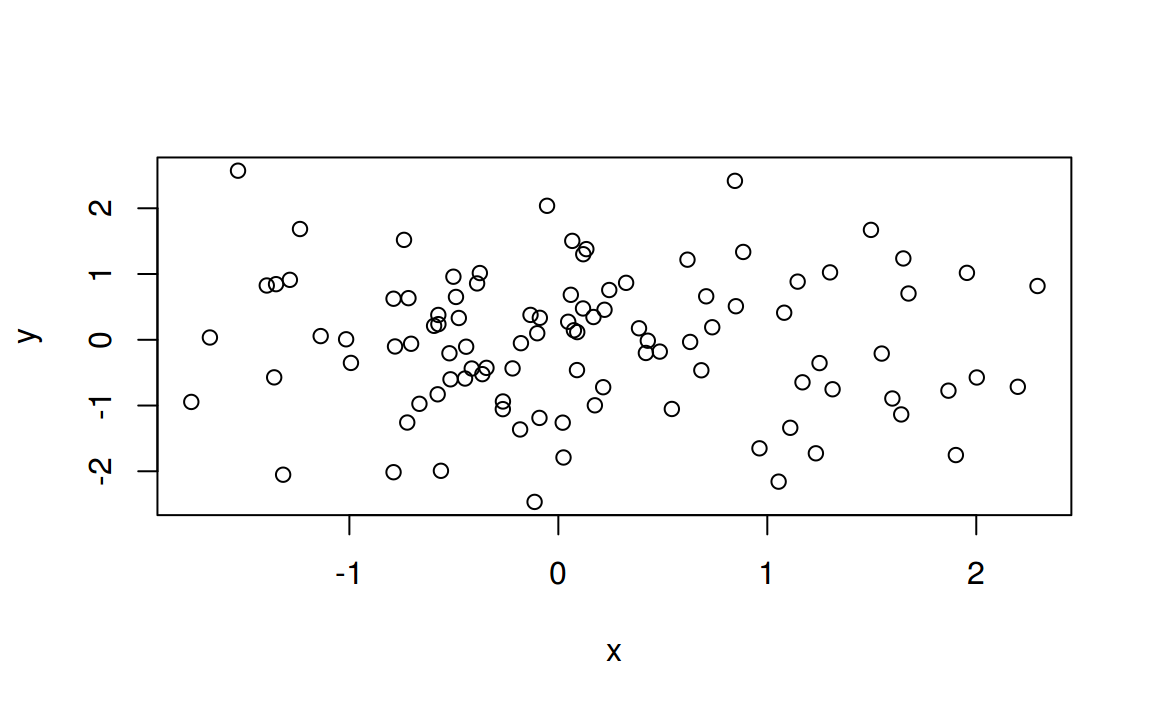
\includegraphics[width=0.7\linewidth]{Machine-Learning_files/figure-latex/unnamed-chunk-15-1} \end{center}

\begin{Shaded}
\begin{Highlighting}[]

\CommentTok{# with titles}
\KeywordTok{plot}\NormalTok{(x,y,}\DataTypeTok{xlab=}\StringTok{"this is the x-axis"}\NormalTok{,}\DataTypeTok{ylab=}\StringTok{"this is the y-axis"}\NormalTok{,}
\DataTypeTok{main=}\StringTok{"Plot of X vs Y"}\NormalTok{)}
\end{Highlighting}
\end{Shaded}

\begin{center}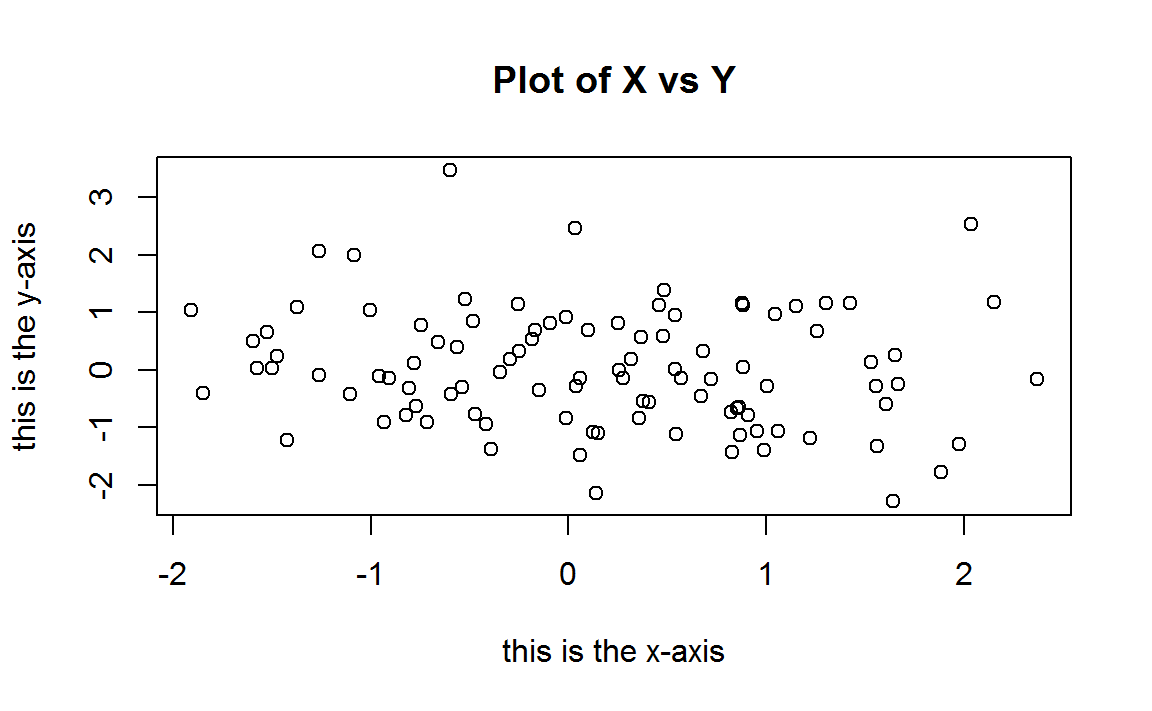
\includegraphics[width=0.7\linewidth]{Machine-Learning_files/figure-latex/unnamed-chunk-15-2} \end{center}

\subsection{Distributions}\label{distributions}

\begin{Shaded}
\begin{Highlighting}[]
\CommentTok{# R allows to sample [r], compute density/probability mass [d],}
\CommentTok{# compute distribution function [p] and compute quantiles [q] for several}
\CommentTok{# continuous and discrete distributions. The format employed is [rdpq]name,}
\CommentTok{# where name stands for:}
\CommentTok{# - norm -> Normal}
\CommentTok{# - unif -> Uniform}
\CommentTok{# - exp -> Exponential}
\CommentTok{# - t -> Student's t}
\CommentTok{# - f -> Snedecor's F (Fisher)}
\CommentTok{# - chisq -> Chi squared}
\CommentTok{# - pois -> Poisson}
\CommentTok{# - binom -> Binomial}
\CommentTok{# More distributions: ?Distributions}


\CommentTok{# Sampling from a Normal - 100 random points from a N(0, 1)}
\KeywordTok{rnorm}\NormalTok{(}\DataTypeTok{n =} \DecValTok{10}\NormalTok{, }\DataTypeTok{mean =} \DecValTok{0}\NormalTok{, }\DataTypeTok{sd =} \DecValTok{1}\NormalTok{)}
\CommentTok{#ans>  [1]  0.189  1.246  1.302 -2.141  0.533 -0.725 -1.291 -1.815 -0.558 -1.132}

\CommentTok{# If you want to have always the same result, set the seed of the random number}
\CommentTok{# generator}
\KeywordTok{set.seed}\NormalTok{(}\DecValTok{45678}\NormalTok{)}
\KeywordTok{rnorm}\NormalTok{(}\DataTypeTok{n =} \DecValTok{10}\NormalTok{, }\DataTypeTok{mean =} \DecValTok{0}\NormalTok{, }\DataTypeTok{sd =} \DecValTok{1}\NormalTok{)}
\CommentTok{#ans>  [1]  1.440 -0.720  0.671 -0.422  0.378 -1.667 -0.508  0.443 -1.799 -0.618}

\CommentTok{# Plotting the density of a N(0, 1) - the Gauss bell}
\NormalTok{x <-}\StringTok{ }\KeywordTok{seq}\NormalTok{(-}\DecValTok{4}\NormalTok{, }\DecValTok{4}\NormalTok{, }\DataTypeTok{l =} \DecValTok{100}\NormalTok{)}
\NormalTok{y <-}\StringTok{ }\KeywordTok{dnorm}\NormalTok{(}\DataTypeTok{x =} \NormalTok{x, }\DataTypeTok{mean =} \DecValTok{0}\NormalTok{, }\DataTypeTok{sd =} \DecValTok{1}\NormalTok{)}
\KeywordTok{plot}\NormalTok{(x, y, }\DataTypeTok{type =} \StringTok{"l"}\NormalTok{)}
\end{Highlighting}
\end{Shaded}

\begin{center}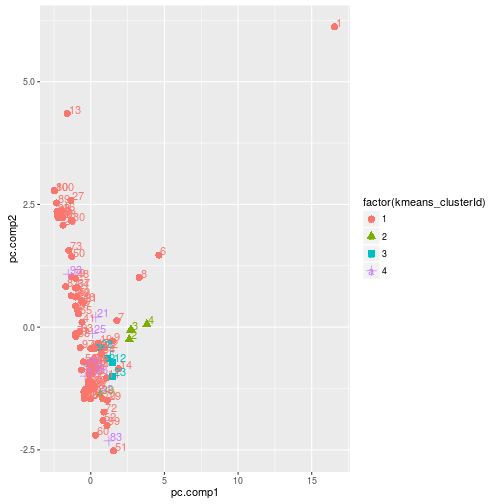
\includegraphics[width=0.7\linewidth]{Machine-Learning_files/figure-latex/unnamed-chunk-16-1} \end{center}

\begin{Shaded}
\begin{Highlighting}[]

\CommentTok{# Plotting the distribution function of a N(0, 1)}
\NormalTok{x <-}\StringTok{ }\KeywordTok{seq}\NormalTok{(-}\DecValTok{4}\NormalTok{, }\DecValTok{4}\NormalTok{, }\DataTypeTok{l =} \DecValTok{100}\NormalTok{)}
\NormalTok{y <-}\StringTok{ }\KeywordTok{pnorm}\NormalTok{(}\DataTypeTok{q =} \NormalTok{x, }\DataTypeTok{mean =} \DecValTok{0}\NormalTok{, }\DataTypeTok{sd =} \DecValTok{1}\NormalTok{)}
\KeywordTok{plot}\NormalTok{(x, y, }\DataTypeTok{type =} \StringTok{"l"}\NormalTok{, }\DataTypeTok{lwd =} \DecValTok{3}\NormalTok{, }\DataTypeTok{main=}\StringTok{"The distribution function of a N(0, 1)"}\NormalTok{)}
\end{Highlighting}
\end{Shaded}

\begin{center}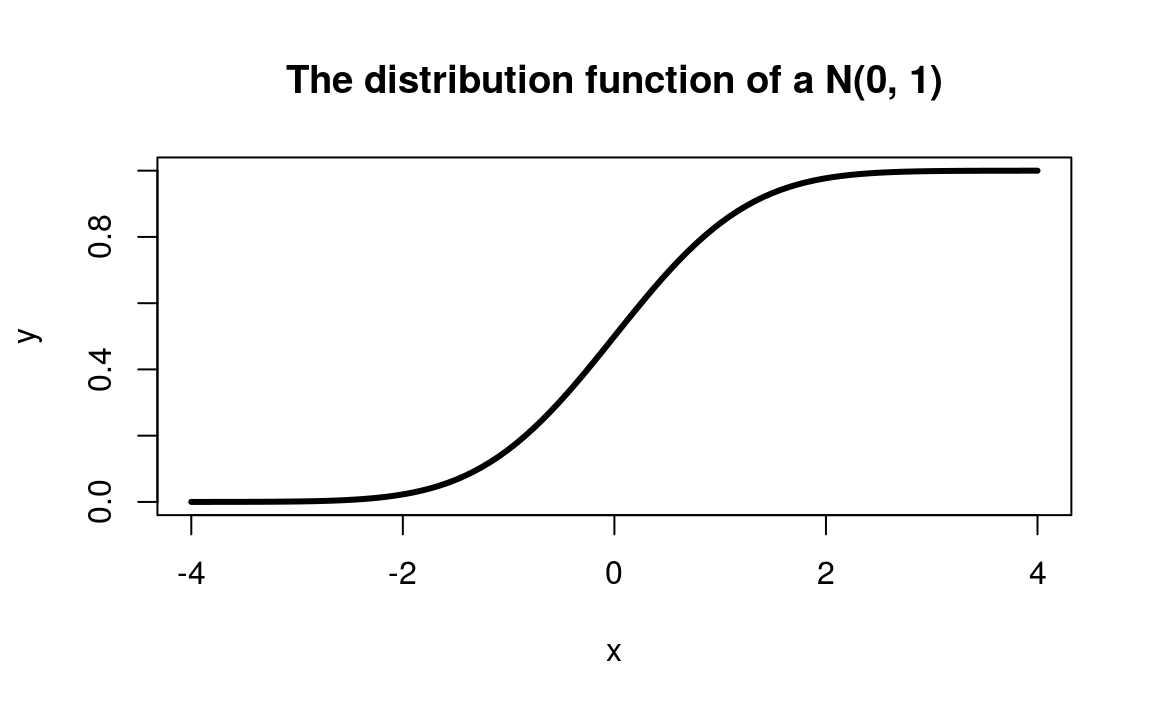
\includegraphics[width=0.7\linewidth]{Machine-Learning_files/figure-latex/unnamed-chunk-16-2} \end{center}

\begin{Shaded}
\begin{Highlighting}[]

\CommentTok{# Computing the 95% quantile for a N(0, 1)}
\KeywordTok{qnorm}\NormalTok{(}\DataTypeTok{p =} \FloatTok{0.95}\NormalTok{, }\DataTypeTok{mean =} \DecValTok{0}\NormalTok{, }\DataTypeTok{sd =} \DecValTok{1}\NormalTok{)}
\CommentTok{#ans> [1] 1.64}

\CommentTok{# All distributions have the same syntax: rname(n,...), dname(x,...), dname(p,...)  }
\CommentTok{# and qname(p,...), but the parameters in ... change. Look them in ?Distributions}
\CommentTok{# For example, here is que same for the uniform distribution}

\CommentTok{# Sampling from a U(0, 1)}
\KeywordTok{set.seed}\NormalTok{(}\DecValTok{45678}\NormalTok{)}
\KeywordTok{runif}\NormalTok{(}\DataTypeTok{n =} \DecValTok{10}\NormalTok{, }\DataTypeTok{min =} \DecValTok{0}\NormalTok{, }\DataTypeTok{max =} \DecValTok{1}\NormalTok{)}
\CommentTok{#ans>  [1] 0.9251 0.3340 0.2359 0.3366 0.7489 0.9327 0.3365 0.2246 0.6474 0.0808}

\CommentTok{# Plotting the density of a U(0, 1)}
\NormalTok{x <-}\StringTok{ }\KeywordTok{seq}\NormalTok{(-}\DecValTok{2}\NormalTok{, }\DecValTok{2}\NormalTok{, }\DataTypeTok{l =} \DecValTok{100}\NormalTok{)}
\NormalTok{y <-}\StringTok{ }\KeywordTok{dunif}\NormalTok{(}\DataTypeTok{x =} \NormalTok{x, }\DataTypeTok{min =} \DecValTok{0}\NormalTok{, }\DataTypeTok{max =} \DecValTok{1}\NormalTok{)}
\KeywordTok{plot}\NormalTok{(x, y, }\DataTypeTok{type =} \StringTok{"l"}\NormalTok{)}
\end{Highlighting}
\end{Shaded}

\begin{center}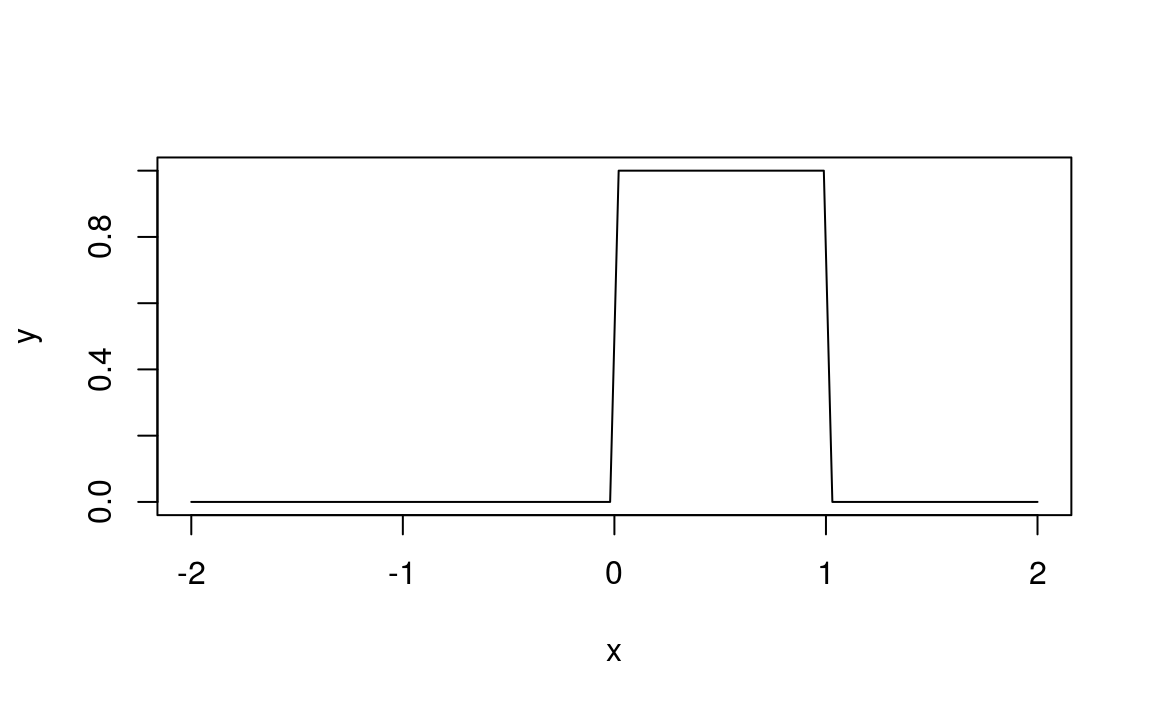
\includegraphics[width=0.7\linewidth]{Machine-Learning_files/figure-latex/unnamed-chunk-16-3} \end{center}

\begin{Shaded}
\begin{Highlighting}[]

\CommentTok{# Computing the 95% quantile for a U(0, 1)}
\KeywordTok{qunif}\NormalTok{(}\DataTypeTok{p =} \FloatTok{0.95}\NormalTok{, }\DataTypeTok{min =} \DecValTok{0}\NormalTok{, }\DataTypeTok{max =} \DecValTok{1}\NormalTok{)}
\CommentTok{#ans> [1] 0.95}
\end{Highlighting}
\end{Shaded}

\begin{rmdexercise}
Do the following:

\begin{itemize}
\tightlist
\item
  Compute the 90\%, 95\% and 99\% quantiles of a \(F\) distribution with
  \texttt{df1\ =\ 1} and \texttt{df2\ =\ 5}. (Answer:
  \texttt{c(4.060420,\ 6.607891,\ 16.258177)})
\item
  Sample 100 points from a Poisson with \texttt{lambda\ =\ 5}.
\item
  Plot the density of a \(t\) distribution with \texttt{df\ =\ 1} (use a
  sequence spanning from \texttt{-4} to \texttt{4}). Add lines of
  different colors with the densities for \texttt{df\ =\ 5},
  \texttt{df\ =\ 10}, \texttt{df\ =\ 50} and \texttt{df\ =\ 100}.
\end{itemize}
\end{rmdexercise}

\subsection{Working directory}\label{working-directory}

Your \emph{working directory} is the folder on your computer in which
you are currently working. When you ask R to open a certain file, it
will look in the working directory for this file, and when you tell R to
save a data file or figure, it will save it in the working directory.

To set your working directory within RStudio you can go to
\texttt{Tools\ /\ Set\ working\ directory}, or use the command
\texttt{setwd()}, we put the complete path of the directory between the
brackets, do not forget to put the path into quotation marks
\texttt{""}.

To know the actual working directory we use \texttt{getwd()}.

\subsection{Loading Data}\label{loading-data}

The \texttt{read.table()} function is one of the primary ways to import
a data set into \texttt{R}. The help file \texttt{?read.table()}
contains details about how to use this function. We can use the function
\texttt{write.table()} to export data.

Next we will show how to load the data set
\href{datasets/Auto.data}{\texttt{Auto.data}}.

\begin{Shaded}
\begin{Highlighting}[]
\NormalTok{Auto=}\KeywordTok{read.table}\NormalTok{(}\StringTok{"Auto.data"}\NormalTok{,}\DataTypeTok{header=}\NormalTok{T,}\DataTypeTok{na.strings =}\StringTok{"?"}\NormalTok{)}
\CommentTok{# For this file we needed to tell R that the first row is the}
\CommentTok{# names of the variables.}
\CommentTok{# na.strings tells R that any time it sees a particular character}
\CommentTok{# or set of characters (such as a question mark), it should be}
\CommentTok{# treated as a missing element of the data matrix. }
\end{Highlighting}
\end{Shaded}

\begin{rmdinsight}
\begin{itemize}
\tightlist
\item
  If the file is of csv format, we use \texttt{read.csv}.
\item
  Always try to look to the file before importing it to \texttt{R} (Open
  it in a text editor. See for example if the first row containes the
  variables names, if the columns are separated by \texttt{,} or
  \texttt{;} or ..
\item
  For text editors, I suggest
  \href{https://www.sublimetext.com/}{\texttt{Sublime\ Text}} or
  \href{https://atom.io/}{\texttt{Atom}}.
\end{itemize}
\end{rmdinsight}

\begin{Shaded}
\begin{Highlighting}[]
\KeywordTok{dim}\NormalTok{(Auto) }\CommentTok{# To see the dimensions of the data set}
\CommentTok{#ans> [1] 397   9}
\KeywordTok{nrow}\NormalTok{(Auto) }\CommentTok{# To see the number of rows}
\CommentTok{#ans> [1] 397}
\KeywordTok{ncol}\NormalTok{(Auto) }\CommentTok{# To see the number of columns}
\CommentTok{#ans> [1] 9}
\NormalTok{Auto[}\DecValTok{1}\NormalTok{:}\DecValTok{4}\NormalTok{,] }\CommentTok{# The first 4 rows of the data set}
\CommentTok{#ans>   mpg cylinders displacement horsepower weight acceleration year origin}
\CommentTok{#ans> 1  18         8          307        130   3504         12.0   70      1}
\CommentTok{#ans> 2  15         8          350        165   3693         11.5   70      1}
\CommentTok{#ans> 3  18         8          318        150   3436         11.0   70      1}
\CommentTok{#ans> 4  16         8          304        150   3433         12.0   70      1}
\CommentTok{#ans>                        name}
\CommentTok{#ans> 1 chevrolet chevelle malibu}
\CommentTok{#ans> 2         buick skylark 320}
\CommentTok{#ans> 3        plymouth satellite}
\CommentTok{#ans> 4             amc rebel sst}
\end{Highlighting}
\end{Shaded}

\begin{Shaded}
\begin{Highlighting}[]
\CommentTok{# Once the data are loaded correctly, we can use names()}
\CommentTok{# to check the variable names.}
\KeywordTok{names}\NormalTok{(Auto)}
\CommentTok{#ans> [1] "mpg"          "cylinders"    "displacement" "horsepower"  }
\CommentTok{#ans> [5] "weight"       "acceleration" "year"         "origin"      }
\CommentTok{#ans> [9] "name"}
\end{Highlighting}
\end{Shaded}

\begin{rmdinsight}
Take a look at this
\href{https://cran.r-project.org/doc/contrib/Torfs+Brauer-Short-R-Intro.pdf}{(very)
short introduction to R}. It can be useful.
\end{rmdinsight}

\section{Regression}\label{regression}

\subsection{\texorpdfstring{The \texttt{lm}
function}{The lm function}}\label{the-lm-function}

We are going to employ the \texttt{EU} dataset. The \texttt{EU} dataset
contains 28 rows with the member states of the European Union (Country),
the number of seats assigned under different years (Seats2011,
Seats2014), the Cambridge Compromise apportionment (CamCom2011), and the
countries population (Population2010,Population2013).

\begin{Shaded}
\begin{Highlighting}[]
\CommentTok{# Load the dataset, when we load an .RData using load()}
\CommentTok{# function we do not attribute it to a name like we did}
\CommentTok{# when we used read.table() or when we use read.csv()}

\KeywordTok{load}\NormalTok{(}\StringTok{"EU.RData"}\NormalTok{)}
\end{Highlighting}
\end{Shaded}

\begin{rmdinsight}
There is two ways to tell \texttt{R}~where is the file you want to
load/use/import or where to save a file when you write/export/save :

\begin{enumerate}
\def\labelenumi{\arabic{enumi}.}
\tightlist
\item
  write the complete path of the files.
\item
  set a working directory and put the files in it.
\end{enumerate}
\end{rmdinsight}

\begin{Shaded}
\begin{Highlighting}[]
\CommentTok{# lm (for linear model) has the syntax: }
\CommentTok{# lm(formula = response ~ predictor, data = data)}
\CommentTok{# The response is the y in the model. The predictor is x.}
\CommentTok{# For example (after loading the EU dataset)}
\NormalTok{mod <-}\StringTok{ }\KeywordTok{lm}\NormalTok{(}\DataTypeTok{formula =} \NormalTok{Seats2011 ~}\StringTok{ }\NormalTok{Population2010, }\DataTypeTok{data =} \NormalTok{EU)}

\CommentTok{# We have saved the linear model into mod, which now contains all the output of lm}
\CommentTok{# You can see it by typing}
\NormalTok{mod}
\CommentTok{#ans> }
\CommentTok{#ans> Call:}
\CommentTok{#ans> lm(formula = Seats2011 ~ Population2010, data = EU)}
\CommentTok{#ans> }
\CommentTok{#ans> Coefficients:}
\CommentTok{#ans>    (Intercept)  Population2010  }
\CommentTok{#ans>       7.91e+00        1.08e-06}

\CommentTok{# mod is indeed a list of objects whose names are}
\KeywordTok{names}\NormalTok{(mod)}
\CommentTok{#ans>  [1] "coefficients"  "residuals"     "effects"       "rank"         }
\CommentTok{#ans>  [5] "fitted.values" "assign"        "qr"            "df.residual"  }
\CommentTok{#ans>  [9] "na.action"     "xlevels"       "call"          "terms"        }
\CommentTok{#ans> [13] "model"}

\CommentTok{# We can access these elements by $}
\CommentTok{# For example}
\NormalTok{mod$coefficients}
\CommentTok{#ans>    (Intercept) Population2010 }
\CommentTok{#ans>       7.91e+00       1.08e-06}

\CommentTok{# The residuals}
\NormalTok{mod$residuals}
\CommentTok{#ans>        Germany         France United Kingdom          Italy          Spain }
\CommentTok{#ans>         2.8675        -3.7031        -1.7847         0.0139        -3.5084 }
\CommentTok{#ans>         Poland        Romania    Netherlands         Greece        Belgium }
\CommentTok{#ans>         1.9272         1.9434         0.2142         1.8977         2.3994 }
\CommentTok{#ans>       Portugal Czech Republic        Hungary         Sweden        Austria }
\CommentTok{#ans>         2.6175         2.7587         3.2898         2.0163         2.0575 }
\CommentTok{#ans>       Bulgaria        Denmark       Slovakia        Finland        Ireland }
\CommentTok{#ans>         1.9328        -0.8790        -0.7606        -0.6813        -0.7284 }
\CommentTok{#ans>      Lithuania         Latvia       Slovenia        Estonia         Cyprus }
\CommentTok{#ans>         0.4998        -1.3347        -2.1175        -3.3552        -2.7761 }
\CommentTok{#ans>     Luxembourg          Malta }
\CommentTok{#ans>        -2.4514        -2.3553}

\CommentTok{# The fitted values}
\NormalTok{mod$fitted.values}
\CommentTok{#ans>        Germany         France United Kingdom          Italy          Spain }
\CommentTok{#ans>          96.13          77.70          74.78          72.99          57.51 }
\CommentTok{#ans>         Poland        Romania    Netherlands         Greece        Belgium }
\CommentTok{#ans>          49.07          31.06          25.79          20.10          19.60 }
\CommentTok{#ans>       Portugal Czech Republic        Hungary         Sweden        Austria }
\CommentTok{#ans>          19.38          19.24          18.71          17.98          16.94 }
\CommentTok{#ans>       Bulgaria        Denmark       Slovakia        Finland        Ireland }
\CommentTok{#ans>          16.07          13.88          13.76          13.68          12.73 }
\CommentTok{#ans>      Lithuania         Latvia       Slovenia        Estonia         Cyprus }
\CommentTok{#ans>          11.50          10.33          10.12           9.36           8.78 }
\CommentTok{#ans>     Luxembourg          Malta }
\CommentTok{#ans>           8.45           8.36}

\CommentTok{# Summary of the model}
\NormalTok{sumMod <-}\StringTok{ }\KeywordTok{summary}\NormalTok{(mod)}
\NormalTok{sumMod}
\CommentTok{#ans> }
\CommentTok{#ans> Call:}
\CommentTok{#ans> lm(formula = Seats2011 ~ Population2010, data = EU)}
\CommentTok{#ans> }
\CommentTok{#ans> Residuals:}
\CommentTok{#ans>    Min     1Q Median     3Q    Max }
\CommentTok{#ans> -3.703 -1.951  0.014  1.980  3.290 }
\CommentTok{#ans> }
\CommentTok{#ans> Coefficients:}
\CommentTok{#ans>                Estimate Std. Error t value Pr(>|t|)    }
\CommentTok{#ans> (Intercept)    7.91e+00   5.66e-01    14.0  2.6e-13 ***}
\CommentTok{#ans> Population2010 1.08e-06   1.92e-08    56.3  < 2e-16 ***}
\CommentTok{#ans> ---}
\CommentTok{#ans> Signif. codes:  0 '***' 0.001 '**' 0.01 '*' 0.05 '.' 0.1 ' ' 1}
\CommentTok{#ans> }
\CommentTok{#ans> Residual standard error: 2.29 on 25 degrees of freedom}
\CommentTok{#ans>   (1 observation deleted due to missingness)}
\CommentTok{#ans> Multiple R-squared:  0.992,   Adjusted R-squared:  0.992 }
\CommentTok{#ans> F-statistic: 3.17e+03 on 1 and 25 DF,  p-value: <2e-16}
\end{Highlighting}
\end{Shaded}

The following table contains a handy cheat sheet of equivalences between
\texttt{R} code and some of the statistical concepts associated to
linear regression.

\begin{longtable}[]{@{}ll@{}}
\toprule
\begin{minipage}[b]{0.49\columnwidth}\raggedright\strut
\texttt{R}\strut
\end{minipage} & \begin{minipage}[b]{0.45\columnwidth}\raggedright\strut
Statistical concept\strut
\end{minipage}\tabularnewline
\midrule
\endhead
\begin{minipage}[t]{0.49\columnwidth}\raggedright\strut
\texttt{x}\strut
\end{minipage} & \begin{minipage}[t]{0.45\columnwidth}\raggedright\strut
Predictor \(X_1,\ldots,X_n\)\strut
\end{minipage}\tabularnewline
\begin{minipage}[t]{0.49\columnwidth}\raggedright\strut
\texttt{y}\strut
\end{minipage} & \begin{minipage}[t]{0.45\columnwidth}\raggedright\strut
Response \(Y_1,\ldots,Y_n\)\strut
\end{minipage}\tabularnewline
\begin{minipage}[t]{0.49\columnwidth}\raggedright\strut
\texttt{data\ \textless{}-\ data.frame(x\ =\ x,\ y\ =\ y)}\strut
\end{minipage} & \begin{minipage}[t]{0.45\columnwidth}\raggedright\strut
Sample \((X_1,Y_1),\ldots,(X_n,Y_n)\)\strut
\end{minipage}\tabularnewline
\begin{minipage}[t]{0.49\columnwidth}\raggedright\strut
\texttt{model\ \textless{}-\ lm(y\ \textasciitilde{}\ x,\ data\ =\ data)}\strut
\end{minipage} & \begin{minipage}[t]{0.45\columnwidth}\raggedright\strut
Fitted linear model\strut
\end{minipage}\tabularnewline
\begin{minipage}[t]{0.49\columnwidth}\raggedright\strut
\texttt{model\$coefficients}\strut
\end{minipage} & \begin{minipage}[t]{0.45\columnwidth}\raggedright\strut
Fitted coefficients \(\hat\beta_0,\hat\beta_1\)\strut
\end{minipage}\tabularnewline
\begin{minipage}[t]{0.49\columnwidth}\raggedright\strut
\texttt{model\$residuals}\strut
\end{minipage} & \begin{minipage}[t]{0.45\columnwidth}\raggedright\strut
Fitted residuals \(\hat\varepsilon_1,\ldots,\hat\varepsilon_n\)\strut
\end{minipage}\tabularnewline
\begin{minipage}[t]{0.49\columnwidth}\raggedright\strut
\texttt{model\$fitted.values}\strut
\end{minipage} & \begin{minipage}[t]{0.45\columnwidth}\raggedright\strut
Fitted values \(\hat Y_1,\ldots,\hat Y_n\)\strut
\end{minipage}\tabularnewline
\begin{minipage}[t]{0.49\columnwidth}\raggedright\strut
\texttt{model\$df.residual}\strut
\end{minipage} & \begin{minipage}[t]{0.45\columnwidth}\raggedright\strut
Degrees of freedom \(n-2\)\strut
\end{minipage}\tabularnewline
\begin{minipage}[t]{0.49\columnwidth}\raggedright\strut
\texttt{summaryModel\ \textless{}-\ summary(model)}\strut
\end{minipage} & \begin{minipage}[t]{0.45\columnwidth}\raggedright\strut
Summary of the fitted linear model\strut
\end{minipage}\tabularnewline
\begin{minipage}[t]{0.49\columnwidth}\raggedright\strut
\texttt{summaryModel\$sigma}\strut
\end{minipage} & \begin{minipage}[t]{0.45\columnwidth}\raggedright\strut
Fitted residual standard deviation \(\hat\sigma\)\strut
\end{minipage}\tabularnewline
\begin{minipage}[t]{0.49\columnwidth}\raggedright\strut
\texttt{summaryModel\$r.squared}\strut
\end{minipage} & \begin{minipage}[t]{0.45\columnwidth}\raggedright\strut
Coefficient of determination \(R^2\)\strut
\end{minipage}\tabularnewline
\begin{minipage}[t]{0.49\columnwidth}\raggedright\strut
\texttt{summaryModel\$fstatistic}\strut
\end{minipage} & \begin{minipage}[t]{0.45\columnwidth}\raggedright\strut
\(F\)-test\strut
\end{minipage}\tabularnewline
\begin{minipage}[t]{0.49\columnwidth}\raggedright\strut
\texttt{anova(model)}\strut
\end{minipage} & \begin{minipage}[t]{0.45\columnwidth}\raggedright\strut
ANOVA table\strut
\end{minipage}\tabularnewline
\bottomrule
\end{longtable}

\begin{rmdexercise}
Do the following:

\begin{itemize}
\tightlist
\item
  Download The `EU' dataset from \href{datasets/EU.RData}{here} as an
  \texttt{.RData} file and load it using the function \texttt{load}.
\item
  Compute the regression of \texttt{CamCom2011} into
  \texttt{Population2010}. Save that model as the variable
  \texttt{myModel}.
\item
  Access the objects \texttt{residuals} and \texttt{coefficients} of
  \texttt{myModel}.
\item
  Compute the summary of \texttt{myModel} and store it as the variable
  \texttt{summaryMyModel}.
\item
  Access the object \texttt{sigma} of \texttt{myModel}.
\end{itemize}
\end{rmdexercise}

\subsection{Predicting House Value: Boston
dataset}\label{predicting-house-value-boston-dataset}

We are going to use a dataset called Boston which is part of the
\texttt{MASS} package. It recordes the median value of houses for 506
neighborhoods around Boston. Our task is to predict the median house
value (\texttt{medv}) using only one predictor (\texttt{lstat}: percent
of households with low socioeconomic status).

\begin{Shaded}
\begin{Highlighting}[]
\CommentTok{# First, install the MASS package using the command: install.packages("MASS")}

\CommentTok{# load MASS package}
\KeywordTok{library}\NormalTok{(MASS)}

\CommentTok{# Check the dimensions of the Boston dataset}
\KeywordTok{dim}\NormalTok{(Boston)}
\CommentTok{#ans> [1] 506  14}
\end{Highlighting}
\end{Shaded}

\textbf{STEP 1: Split the dataset}

\begin{Shaded}
\begin{Highlighting}[]
\CommentTok{# Split the data by using the first 400 observations as the training}
\CommentTok{# data and the remaining as the testing data}
\NormalTok{train =}\StringTok{ }\DecValTok{1}\NormalTok{:}\DecValTok{400}
\NormalTok{test =}\StringTok{ }\NormalTok{-train}

\CommentTok{# Speficy that we are going to use only two variables (lstat and medv)}
\NormalTok{variables =}\StringTok{ }\KeywordTok{which}\NormalTok{(}\KeywordTok{names}\NormalTok{(Boston) ==}\KeywordTok{c}\NormalTok{(}\StringTok{"lstat"}\NormalTok{, }\StringTok{"medv"}\NormalTok{))}
\NormalTok{training_data =}\StringTok{ }\NormalTok{Boston[train, variables]}
\NormalTok{testing_data =}\StringTok{ }\NormalTok{Boston[test, variables]}

\CommentTok{# Check the dimensions of the new dataset}
\KeywordTok{dim}\NormalTok{(training_data)}
\CommentTok{#ans> [1] 400   2}
\end{Highlighting}
\end{Shaded}

\textbf{STEP 2: Check for Linearity}

In order to perfom linear regression in \texttt{R}, we will use the
function \texttt{lm()}to fit a simple linear regression with
\texttt{medv} as the response (dependent variable) and \texttt{lstat} as
the predictor or independent variable, and then save it in
\texttt{model}.

But before we run our model, let's visually check if the relationship
between x and y is linear.

\begin{Shaded}
\begin{Highlighting}[]
\CommentTok{# Scatterplot of lstat vs. medv}
\KeywordTok{plot}\NormalTok{(training_data$lstat, training_data$medv)}
\end{Highlighting}
\end{Shaded}

\begin{center}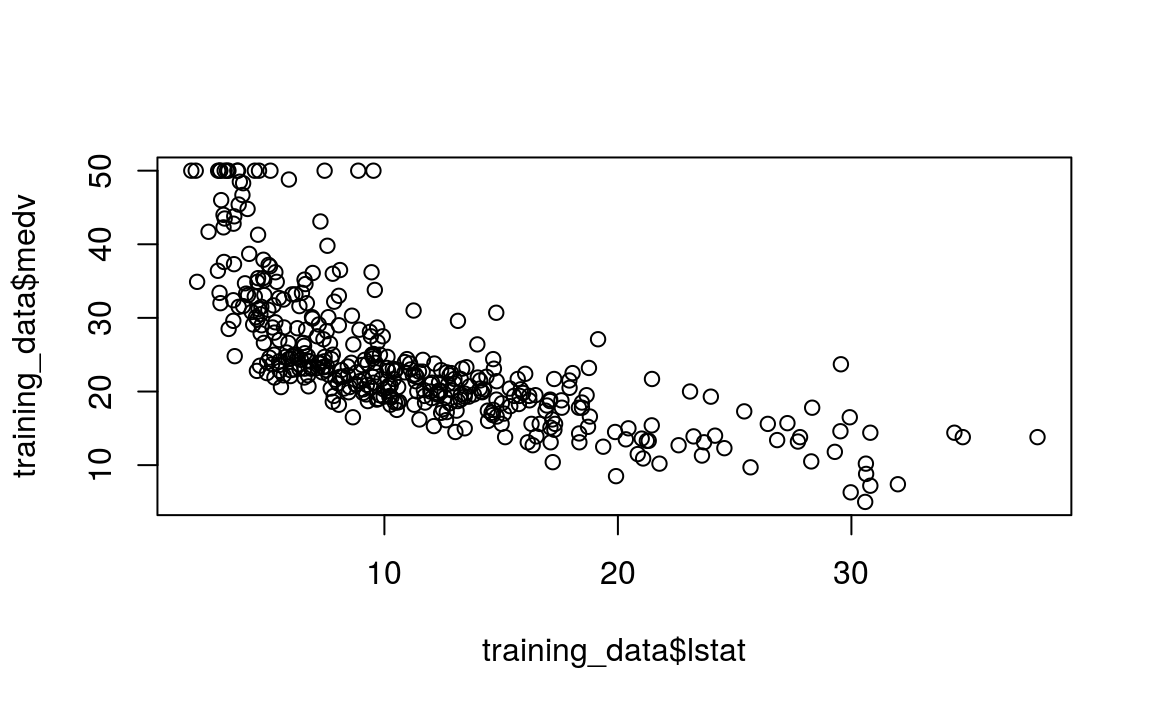
\includegraphics[width=0.7\linewidth]{Machine-Learning_files/figure-latex/unnamed-chunk-31-1} \end{center}

According to the plot, we see that the relationship is not linear. Let's
try a transformation of our explanatory variable \texttt{lstat}.

\begin{Shaded}
\begin{Highlighting}[]
\CommentTok{# Scatterplot of log(lstat) vs. medv}
\KeywordTok{plot}\NormalTok{(}\KeywordTok{log}\NormalTok{(training_data$lstat), training_data$medv)}
\end{Highlighting}
\end{Shaded}

\begin{center}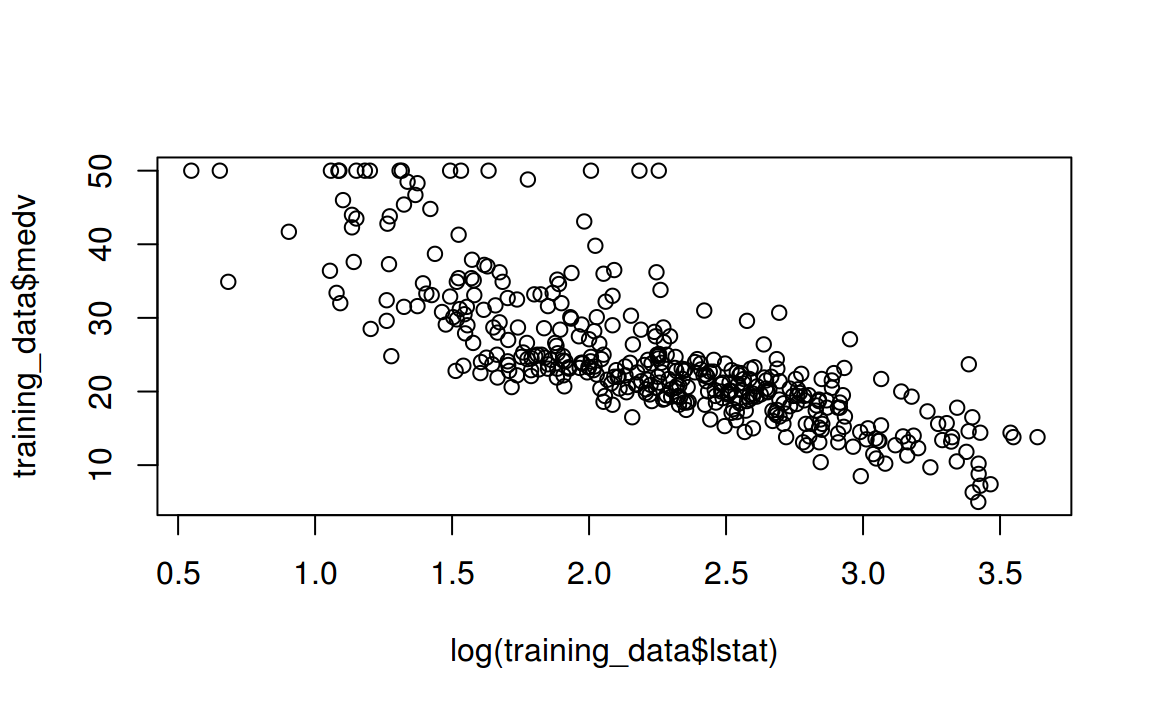
\includegraphics[width=0.7\linewidth]{Machine-Learning_files/figure-latex/unnamed-chunk-32-1} \end{center}

Look at the plot, it is more linear, so we can proceed and perform
\texttt{lm()}:

\textbf{STEP 3: Run the linear regression model}

\begin{Shaded}
\begin{Highlighting}[]
\NormalTok{model =}\StringTok{ }\KeywordTok{lm}\NormalTok{(medv ~}\StringTok{ }\KeywordTok{log}\NormalTok{(lstat), }\DataTypeTok{data =} \NormalTok{training_data)}
\NormalTok{model}
\CommentTok{#ans> }
\CommentTok{#ans> Call:}
\CommentTok{#ans> lm(formula = medv ~ log(lstat), data = training_data)}
\CommentTok{#ans> }
\CommentTok{#ans> Coefficients:}
\CommentTok{#ans> (Intercept)   log(lstat)  }
\CommentTok{#ans>        51.8        -12.2}
\end{Highlighting}
\end{Shaded}

Notice that basic information when we print \texttt{model}. This only
give us the slope \((-12.2)\) and the intercept \((51.8)\) of the linear
model. Note that here we are looking at \texttt{log(lstat)} and not
\texttt{lstat} anymore. So for every one unit increase in
\texttt{lstat}, the median value of the house will decrease by
\(e^{12.2}\). For more detailed information, we can use the
\texttt{summary()} function:

\begin{Shaded}
\begin{Highlighting}[]
\KeywordTok{summary}\NormalTok{(model)}
\CommentTok{#ans> }
\CommentTok{#ans> Call:}
\CommentTok{#ans> lm(formula = medv ~ log(lstat), data = training_data)}
\CommentTok{#ans> }
\CommentTok{#ans> Residuals:}
\CommentTok{#ans>     Min      1Q  Median      3Q     Max }
\CommentTok{#ans> -11.385  -3.908  -0.779   2.245  25.728 }
\CommentTok{#ans> }
\CommentTok{#ans> Coefficients:}
\CommentTok{#ans>             Estimate Std. Error t value Pr(>|t|)    }
\CommentTok{#ans> (Intercept)   51.783      1.097    47.2   <2e-16 ***}
\CommentTok{#ans> log(lstat)   -12.203      0.472   -25.9   <2e-16 ***}
\CommentTok{#ans> ---}
\CommentTok{#ans> Signif. codes:  0 '***' 0.001 '**' 0.01 '*' 0.05 '.' 0.1 ' ' 1}
\CommentTok{#ans> }
\CommentTok{#ans> Residual standard error: 5.6 on 398 degrees of freedom}
\CommentTok{#ans> Multiple R-squared:  0.627,   Adjusted R-squared:  0.626 }
\CommentTok{#ans> F-statistic:  669 on 1 and 398 DF,  p-value: <2e-16}
\end{Highlighting}
\end{Shaded}

Now, we have access to p-values and standard errors for the
coefficients, as well as the \(R^2\).

\begin{itemize}
\tightlist
\item
  The output states that the slope is statistically significant and
  different from \(0\) and with a t-value= \(-25.9\) (p-value
  \(< 0.05\)), which means that there is a significant relationship
  between the percentage of households with low socioeconomic income and
  the median house value.
\item
  This relationship is negative. That is as the percantage of household
  with low socioeconomic income increases, the median house value
  decreases.
\item
  Looking at \(R^2\), we can deduce that \(62.7\%\) of the model
  variation is being explained by the predictor \texttt{log(lstat)}.
  This is probably low, but indeed it would increase if we had more
  independent (explanatory) variables. We can use the \texttt{names()}
  function to see what other pieces of information are stored in our
  linear model (\texttt{model}).
\end{itemize}

\begin{Shaded}
\begin{Highlighting}[]
\KeywordTok{names}\NormalTok{(model)}
\CommentTok{#ans>  [1] "coefficients"  "residuals"     "effects"       "rank"         }
\CommentTok{#ans>  [5] "fitted.values" "assign"        "qr"            "df.residual"  }
\CommentTok{#ans>  [9] "xlevels"       "call"          "terms"         "model"}
\end{Highlighting}
\end{Shaded}

\begin{Shaded}
\begin{Highlighting}[]
\NormalTok{model$coefficients}
\CommentTok{#ans> (Intercept)  log(lstat) }
\CommentTok{#ans>        51.8       -12.2}
\end{Highlighting}
\end{Shaded}

To obtain the confidence intervel for the linear model (\texttt{model}),
we can use the \texttt{confint()} function:

\begin{Shaded}
\begin{Highlighting}[]
\KeywordTok{confint}\NormalTok{(model, }\DataTypeTok{level =} \FloatTok{0.95}\NormalTok{)}
\CommentTok{#ans>             2.5 % 97.5 %}
\CommentTok{#ans> (Intercept)  49.6   53.9}
\CommentTok{#ans> log(lstat)  -13.1  -11.3}
\end{Highlighting}
\end{Shaded}

So, a \(95\%\) confidence interval for the slope of \texttt{log(lstat)}
is \((-13.13, -11.28)\). Notice that this confidence interval gives us
the same result as the hypothesis test performed earlier, by stating
that we are \(95\%\) confident that the slope of \texttt{lstat} is not
zero (in fact it is less than zero, which means that the relationship is
negative.)

\textbf{STEP 4: Plot the regression model}

Now, let's plot our regression line on top of our data.

\begin{Shaded}
\begin{Highlighting}[]
\CommentTok{# Scatterplot of lstat vs. medv}
\KeywordTok{plot}\NormalTok{(}\KeywordTok{log}\NormalTok{(training_data$lstat), training_data$medv)}

\CommentTok{# Add the regression line to the existing scatterplot}
\KeywordTok{abline}\NormalTok{(model)}
\end{Highlighting}
\end{Shaded}

\begin{center}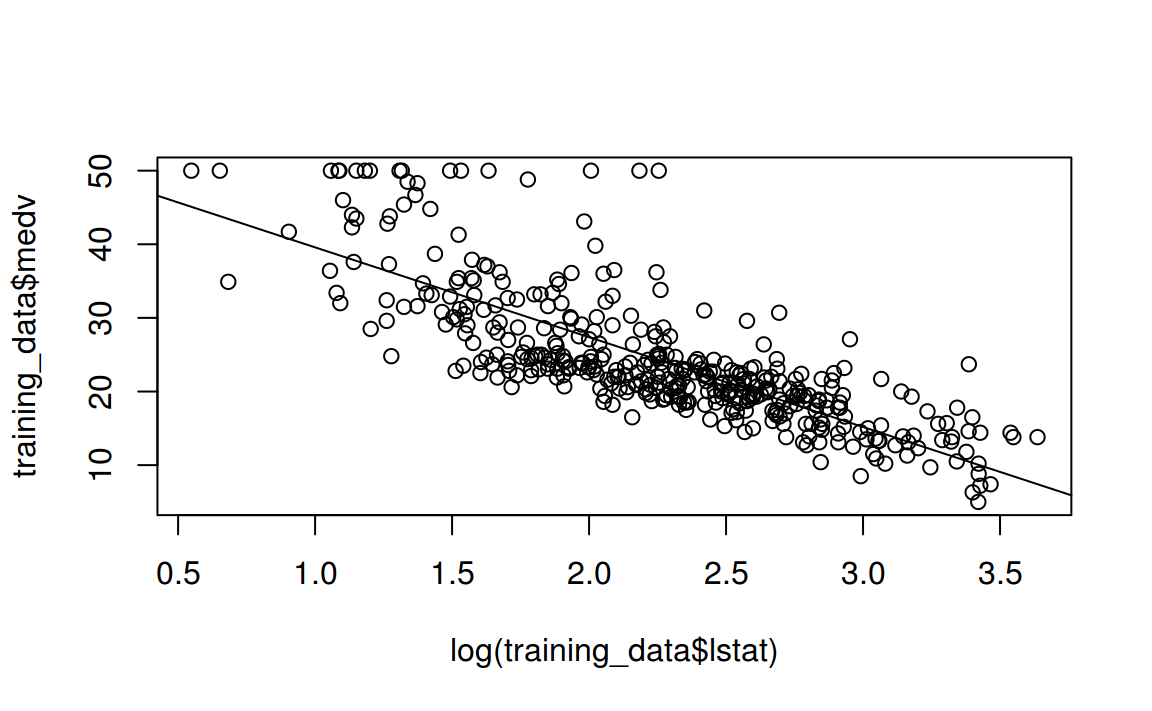
\includegraphics[width=0.7\linewidth]{Machine-Learning_files/figure-latex/unnamed-chunk-38-1} \end{center}

Let's play with the look of the plot, and makes it perttier!

\begin{Shaded}
\begin{Highlighting}[]
\CommentTok{# Scatterplot of lstat vs. medv}
\KeywordTok{plot}\NormalTok{(}\KeywordTok{log}\NormalTok{(training_data$lstat), training_data$medv,}
\DataTypeTok{xlab =} \StringTok{"Log Transform of % of Houshold with Low Socioeconomic Income"}\NormalTok{,}
\DataTypeTok{ylab =} \StringTok{"Median House Value"}\NormalTok{,}
\DataTypeTok{col =} \StringTok{"red"}\NormalTok{,}
\DataTypeTok{pch =} \DecValTok{20}\NormalTok{)}

\CommentTok{# Make the line color blue, and the line's width =3 (play with the width!)}
\KeywordTok{abline}\NormalTok{(model, }\DataTypeTok{col =} \StringTok{"blue"}\NormalTok{, }\DataTypeTok{lwd =}\DecValTok{3}\NormalTok{)}
\end{Highlighting}
\end{Shaded}

\begin{center}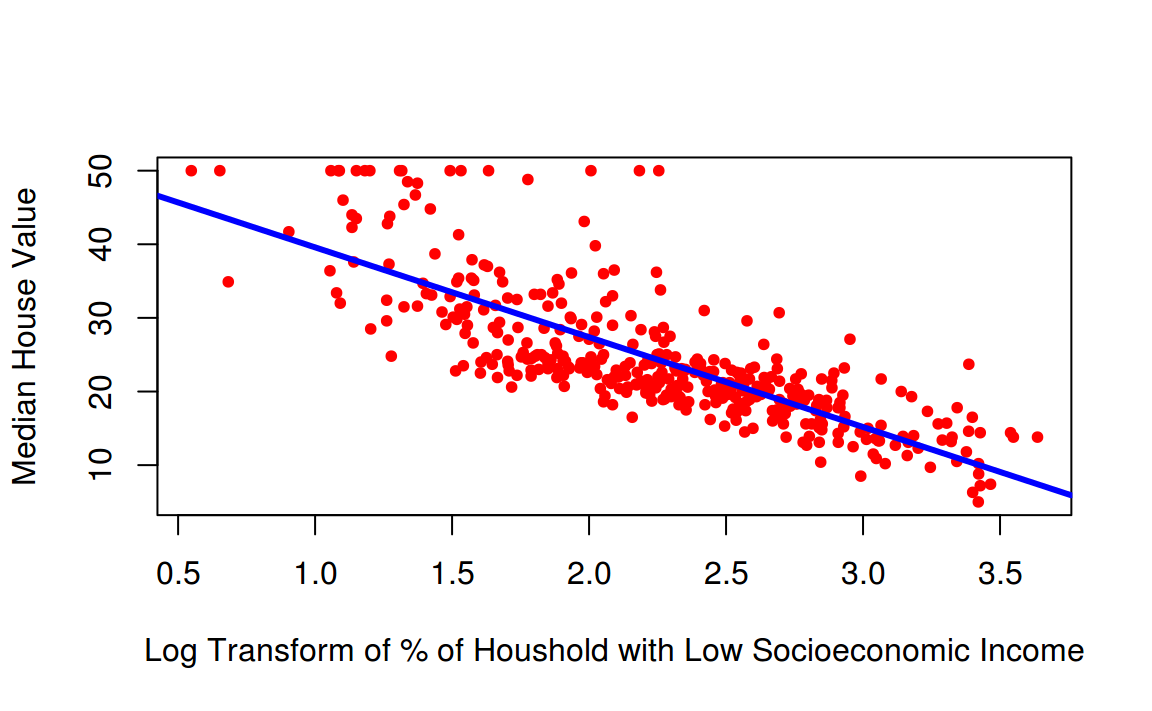
\includegraphics[width=0.7\linewidth]{Machine-Learning_files/figure-latex/unnamed-chunk-39-1} \end{center}

\textbf{STEP 5: Assess the model}

Final thing we will do is to predict using our fitted model. We can use
the \texttt{predict()} function for this purpose:

\begin{Shaded}
\begin{Highlighting}[]
\CommentTok{# Predict what is the median value of the house with lstat= 5%}
\KeywordTok{predict}\NormalTok{(model, }\KeywordTok{data.frame}\NormalTok{(}\DataTypeTok{lstat =} \KeywordTok{c}\NormalTok{(}\DecValTok{5}\NormalTok{)))}
\CommentTok{#ans>    1 }
\CommentTok{#ans> 32.1}
\end{Highlighting}
\end{Shaded}

\begin{Shaded}
\begin{Highlighting}[]
\CommentTok{# Predict what is the median values of houses with lstat= 5%, 10%, and 15%}
\KeywordTok{predict}\NormalTok{(model, }\KeywordTok{data.frame}\NormalTok{(}\DataTypeTok{lstat =} \KeywordTok{c}\NormalTok{(}\DecValTok{5}\NormalTok{,}\DecValTok{10}\NormalTok{,}\DecValTok{15}\NormalTok{), }\DataTypeTok{interval =} \StringTok{"prediction"}\NormalTok{))}
\CommentTok{#ans>    1    2    3 }
\CommentTok{#ans> 32.1 23.7 18.7}
\end{Highlighting}
\end{Shaded}

Now let's assess our model, by computing th mean squared error (MSE). To
assess the model we created, then we will be using the test data!

\begin{Shaded}
\begin{Highlighting}[]
\CommentTok{# Save the testing median values for houses (testing y) in y}
\NormalTok{y =}\StringTok{ }\NormalTok{testing_data$medv}

\CommentTok{# Compute the predicted value for this y (y hat)}
\NormalTok{y_hat =}\StringTok{ }\KeywordTok{predict}\NormalTok{(model, }\KeywordTok{data.frame}\NormalTok{(}\DataTypeTok{lstat =} \NormalTok{testing_data$lstat))}

\CommentTok{# Now we have both y and y_hat for our testing data. }
\CommentTok{# let's find the mean square error}
\NormalTok{error =}\StringTok{ }\NormalTok{y-y_hat}
\NormalTok{error_squared =}\StringTok{ }\NormalTok{error^}\DecValTok{2}
\NormalTok{MSE =}\StringTok{ }\KeywordTok{mean}\NormalTok{(error_squared)}
\NormalTok{MSE}
\CommentTok{#ans> [1] 17.7}
\end{Highlighting}
\end{Shaded}

◼

\chapter{Multiple Linear Regression}\label{multiple-linear-regression}

Simple linear regression is a useful approach for predicting a response
on the basis of a single predictor variable. However, in practice we
often have more than one predictor. In the previous chapter, we took for
example the prediction of housing prices considering we had the size of
each house. We had a single feature \(X\), the size of the house. But
now imagine if we had not only the size of the house as a feature but we
also knew the number of bedrooms, the number of flours and the age of
the house in years. It seems like this would give us a lot more
information with which to predict the price.

\section{The Model}\label{the-model}

In general, suppose that we have \(p\) distinct predictors. Then the
multiple linear regression model takes the form

\[ Y = \beta_0 + \beta_1 X_1 + \beta_2 X_2 + \dots + \beta_p X_p + \epsilon \]

where \(X_j\) represents the \(j\)th predictor and \(\beta_j\)
quantifies the association between that variable and the response. We
interpret \(\beta_j\) as the average effect on \(Y\) of a one unit
increase in \(X_j\), \emph{holding all other predictors fixed}.

In matrix terms, supposing we have \(n\) observations and \(p\)
variables, we need to define the following matrices:

\begin{equation}
 \textbf{Y}_{n \times 1} = \begin{pmatrix}
    Y_{1} \\
    Y_{2} \\
    \vdots \\
    Y_{n}
\end{pmatrix}   \,\,\,\,\,\,\,\,\,\,\,\,  \textbf{X}_{n \times (p+1)}  = \begin{pmatrix}
    1      & X_{11} & X_{12} & \dots  & X_{1p} \\
    1      & X_{21} & X_{22} & \dots  & X_{2p} \\
    \vdots & \vdots & \vdots & \ddots & \vdots \\
    1      & X_{n1} & X_{n2} & \dots  & X_{np}
\end{pmatrix}
\end{equation}

\begin{equation}
 {\mathbb{\beta}}_{(p+1) \times 1} = \begin{pmatrix}
    \beta_{0} \\
    \beta_{1} \\
    \vdots \\
    \beta_{p}
    \end{pmatrix}   \,\,\,\,\,\,\,\,\,\,\,\,  {\epsilon}_{n \times 1} = \begin{pmatrix}
        \epsilon_{1} \\
        \epsilon_{2} \\
        \vdots \\
        \epsilon_{n}
    \end{pmatrix}
\end{equation}

In matrix terms, the general linear regression model is

\[ \textbf{Y}_{n \times 1} = \textbf{X}_{n \times (p+1)} {\mathbb{\beta}}_{(p+1) \times 1} + {\epsilon}_{n \times 1} \]

where,

\begin{itemize}
\tightlist
\item
  \(\textbf{Y}\) is a vector of responses.
\item
  \(\mathbb{\beta}\) is a vector of parameters.
\item
  \(\textbf{X}\) is a matrix of constants.
\item
  \(\epsilon\) is a vector of independent \emph{normal} (Gaussian)
  random variables.
\end{itemize}

\section{Estimating the Regression
Coefficients}\label{estimating-the-regression-coefficients}

As was the case in the simple linear regression setting, the regression
coefficients \(\beta_{0}, \beta_{1}, \ldots, \beta_{p}\) are unknown,
and must be estimated. Given estimates
\(\hat{\beta_{0}}, \hat{\beta_{1}}, \ldots, \hat{\beta_{p}}\), we can
make predictions using the formula

\[ \hat{y} = \hat{\beta_{0}} + \hat{\beta_{1}} x_1 + \hat{\beta_{2}} x_2 + \ldots, \hat{\beta_{p}} x_p \]

We choose \(\beta_{0}, \beta_{1}, \ldots, \beta_{p}\) to minimize the
sum of squared residuals

\[ \begin{aligned}
RSS &= \sum_{i=1}^{n} (y_i - \hat{y}_i)^2 \\
    &= \sum_{i=1}^{n} (y_1 - \hat{\beta_0} - \hat{\beta_1} \hat{x}_{i1}  - \hat{\beta_2} \hat{x}_{i2} - \ldots  -  \hat{\beta_p} \hat{x}_{ip})^2 \\
\end{aligned}
\]

The values \(\hat{\beta_{0}}, \hat{\beta_{1}}, \ldots, \hat{\beta_{p}}\)
that minimize the RSS are the multiple least squares regression
coefficient estimates, they are calculated using this formula (in matrix
terms):

\[ \hat{\beta} = (\textbf{X}^T \textbf{X})^{-1}\textbf{X}^T \textbf{Y} \]

Note 1:

\begin{rmdinsight}
It is a remarkable property of matrix algebra that the results for the
general linear regression model in matrix notation appear exactly as
those for the simple linear regression model. Only the degrees of
freedom and other constants related to the number of \(X\) variables and
the dimensions of some matrices are different.
\end{rmdinsight}

Note 2:

\begin{rmdinsight}
If \(\textbf{X}^T \textbf{X}\) is noninvertible, the common causes might
be having:

\begin{itemize}
\tightlist
\item
  Redundant features, where two features are very closely related
  (i.e.~they are linearly dependent)
\item
  Too many features (e.g. \(p \geq n\)). In this case, we delete some
  features or we use ``regularization'' (to be, maybe, explained in a
  later lesson).
\end{itemize}
\end{rmdinsight}

\section{Some important questions}\label{some-important-questions}

When we perform multiple linear regression, we usually are interested in
answering a few important questions.

\begin{enumerate}
\def\labelenumi{\arabic{enumi}.}
\tightlist
\item
  Is at least one of the predictors \(X_1 ,X_2 ,\ldots,X_p\) useful in
  predicting the response?
\item
  Do all the predictors help to explain \(Y\), or is only a subset of
  the predictors useful?
\item
  How well does the model fit the data?
\item
  Given a set of predictor values, what response value should we
  predict, and how accurate is our prediction?
\end{enumerate}

\textbf{\emph{Relationship Between the Response and Predictors?}}

\textbf{\(F\)-Statistic}

Recall that in the simple linear regression setting, in order to
determine whether there is a relationship between the response and the
predictor we can simply check whether \(\beta_1 = 0\). In the multiple
regression setting with \(p\) predictors, we need to ask whether all of
the regression coefficients are zero, i.e.~whether
\(\beta_1 = \beta_2 = \ldots = \beta_p = 0\). As in the simple linear
regression setting, we use a hypothesis test to answer this question. We
test the null hypothesis,

\[ H_0 : \beta_1 = \beta_2 = \ldots = \beta_p = 0 \]

versus the alternative hypothesis

\[ H_1 : \text{at least one} \, \beta_j \, \text{is non-zero} \]

This hypothesis test is performed by computing the \(F\)-statistic
(\emph{Fisher}):

\[ F = \frac{ (\text{TSS} - \text{RSS})/p}{\text{RSS}/(n-p-1)} \sim F_{p,n-p-1} \]

where, as with simple linear regression,
\(\text{TSS} = \sum (y_i - \bar{y})^2\) and
\(\text{RSS} = \sum (y_i - \hat{y}_i)^2\).

When the \(F\)-statistic value is close to 1, then \(H_0\) is true,
which means there is no relationship between the response and
predictors. On the other hand, if \(H_1\) is true, so we expect \(F\) to
be greater than 1.

So the question we ask here: \emph{Is the whole regression explaining
anything at all?} The answer comes from the \(F\)-test in the ANOVA
(ANalysis Of VAriance) table. This is what we get in an ANOVA table:

\begin{longtable}[]{@{}llllll@{}}
\toprule
Source & df & SS & MS & \(F\) & p-value\tabularnewline
\midrule
\endhead
Factor (Explained) & \(p-1\) & SST & SST/\((k-1)\) & MST/MSE &
p-value\tabularnewline
Error (Unexplained) & \(n-p\) & SSE & SSE/\((n-k)\) & &\tabularnewline
Total & \(n-1\) & SS & & &\tabularnewline
\bottomrule
\end{longtable}

The ANOVA table has many pieces of information. What we care about is
the \(F\) Ratio and the corresponding p-value. We compare the \(F\)
Ratio with \(F_{(p-1,n-p)}\) and a corresponding \(\alpha\) value
(error).

\textbf{p-values}

The p-values provide information about whether each individual predictor
is related to the response, after adjusting for the other predictors.
Let's look at the following table we obtain in general using a
statistical software for example

\begin{longtable}[]{@{}lllll@{}}
\toprule
& Coefficient & Std. error & \(t\)-statistic & p-value\tabularnewline
\midrule
\endhead
Constant & 2.939 & 0.3119 & 9.42 & \textless{}0.0001\tabularnewline
\(X_1\) & 0.046 & 0.0014 & 32.81 & \textless{}0.0001\tabularnewline
\(X_2\) & 0.189 & 0.0086 & 21.89 & \textless{}0.0001\tabularnewline
\(X_3\) & -0.001 & 0.0059 & -0.18 & 0.8599\tabularnewline
\bottomrule
\end{longtable}

In this tablewe the following model

\[ Y = 2.939 + 0.046 X_1 + 0.189 X_2 - 0.001 X_3 \]

Note that for each individual predictor a \(t\)-statistic and a p-value
were reported. These p-values indicate that \(X_1\) and \(X_2\) are
related to \(Y\), but that there is no evidence that \(X_3\) is
associated with \(Y\), in the presence of these two.

\textbf{\emph{Deciding on Important Variables}}

The most direct approach is called \emph{all subsets} or \emph{best
subsets} regression: we compute the least squares fit for all possible
subsets and then choose between them based on some criterion that
balances training error with model size.

However we often can't examine all possible models, since they are
\(2^p\) of them; for example when \(p = 40\) there are over a billion
models! Instead we need an automated approach that searches through a
subset of them. Here are two commonly use approaches:

\textbf{Forward selection}:

\begin{itemize}
\tightlist
\item
  Begin with the \emph{null model} --- a model that contains an
  intercept (constant) but no predictors.
\item
  Fit p simple linear regressions and add to the null model the variable
  that results in the lowest RSS.
\item
  Add to that model the variable that results in the lowest RSS amongst
  all two-variable models.
\item
  Continue until some stopping rule is satisfied, for example when all
  remaining variables have a p-value above some threshold.
\end{itemize}

\textbf{Backward selection}:

\begin{itemize}
\tightlist
\item
  Start with all variables in the model.
\item
  Remove the variable with the largest p-value --- that is, the variable
  that is the least statistically significant.
\item
  The new \((p − 1)\)-variable model is fit, and the variable with the
  largest p-value is removed.
\item
  Continue until a stopping rule is reached. For instance, we may stop
  when all remaining variables have a significant p-value defined by
  some significance threshold.
\end{itemize}

\begin{rmdinsight}
There are more systematic criteria for choosing an ``optimal'' member in
the path of models produced by forward or backward stepwise selection.
These include \emph{Mallow's \(C_p\)} , \emph{Akaike information
criterion (AIC)}, \emph{Bayesian information criterion (BIC)},
\emph{adjusted \(R^2\)} and \emph{Cross-validation (CV)}.
\end{rmdinsight}

\textbf{\emph{Model Fit}}

Two of the most common numerical measures of model fit are the RSE and
\(R^2\), the fraction of variance explained. These quantities are
computed and interpreted in the same fashion as for simple linear
regression. Recall that in simple regression, \(R^2\) is the square of
the correlation of the response and the variable. In multiple linear
regression, it turns out that it equals \(Cor(Y, \hat{Y})^2\) , the
square of the correlation between the response and the fitted linear
model; in fact one property of the fitted linear model is that it
maximizes this correlation among all possible linear models. An \(R^2\)
value close to 1 indicates that the model explains a large portion of
the variance in the response variable.

In general RSE is defined as

\[ \text{RSE} = \sqrt{\frac{1}{n-p-1}\text{RSS}} \]

\subsection{Other Considerations in Regression
Model}\label{other-considerations-in-regression-model}

\textbf{Qualitative Predictors}

\begin{itemize}
\tightlist
\item
  If we have a categorial (qualitative) variable (feature), how do we
  fit into a regression equation?
\item
  For example, if \(X_1\) is the gender (male or female).
\item
  We can code, for example, male = 0 and female = 1.
\item
  Suppose \(X_2\) is a quantitative variable, the regression equation
  becomes:
\end{itemize}

\[ Y_i \approx \beta_0 + \beta_1 X_1 + \beta_2 X_2 = \begin{cases}
  \beta_0 + \beta_2 X_2 & \text{ if male} \\
  \beta_0 + \beta_1 X_1 + \beta_2 X_2 & \text{ if female}
\end{cases} \]

\begin{itemize}
\tightlist
\item
  Another possible coding scheme is to let male = -1 and female = 1, the
  regression equation is then:
\end{itemize}

\[ Y_i \approx \beta_0 + \beta_1 X_1 + \beta_2 X_2 = \begin{cases}
  \beta_0 -\beta_1 X_1 + \beta_2 X_2 & \text{ if male} \\
  \beta_0 + \beta_1 X_1 + \beta_2 X_2 & \text{ if female}
\end{cases} \]

\textbf{Interaction Terms}

\begin{itemize}
\tightlist
\item
  When the effect on \(Y\) of increasing \(X_1\) depends on another
  \(X_2\).
\item
  We may in this case try the model
\end{itemize}

\[ Y_i = \beta_0 + \beta_1 X_1 + \beta_2 X_2 + \beta_3 X_1 X_2 \]

\begin{itemize}
\tightlist
\item
  \(X_1 X_2\) is the Interaction term.
\end{itemize}

◼

\chapter*{PW 2}\label{pw-2}
\addcontentsline{toc}{chapter}{PW 2}

\section{Reporting}\label{reporting}

\subsection*{Markdown}\label{markdown}
\addcontentsline{toc}{subsection}{Markdown}

Markdown is a lightweight markup language with plain text formatting
syntax designed so that it can be converted to HTML and many other
formats (pdf, docx, etc..).

Click \href{http://agea.github.io/tutorial.md/}{here} to see an example
of a markdown (\texttt{.md}) syntaxes and the result in HTML. The
markdown syntaxes are on right and their HTML result is on left. You can
modify the source text to see the result.

\begin{rmdtip}
\textbf{Extra}: There is some markdown online editors you can use, like
\href{http://dillinger.io/}{dillinger.io/}. See the Markdown source file
and the HTML preview. Play with the source text to see the result in the
preview.
\end{rmdtip}

\subsection*{R Markdown}\label{r-markdown}
\addcontentsline{toc}{subsection}{R Markdown}

R Markdown is a variant of Markdown that has embedded \texttt{R} code
chunks, to be used with the \texttt{knitr} package to make it
\textbf{easy to create reproducible web-based reports}.

First, in \texttt{Rstudio} create a new \texttt{R\ Markdown} file. A
default template will be opened. There is some \texttt{R} code in
\texttt{R\ chunks}. Clink on \texttt{knit}, save your file and see the
produced output. The output is a html report containing the results of
the \texttt{R} codes. If your file is named \texttt{report.Rmd}, your
report is named \texttt{report.html}.

\begin{rmdcaution}
\begin{itemize}
\tightlist
\item
  Make sure to have the latest version of \texttt{Rstudio}.
\item
  If you have problems creating a \texttt{R\ Markdown}~file (problem in
  installing packages, etc..) close your \texttt{Rstudio} and reopen it
  with administrative tools and retry.
\item
  If it doesn't work and in order to not lose more time, write your
  script in an \texttt{.R}~file with your comments and submit it.
\end{itemize}
\end{rmdcaution}

\begin{rmdcaution}
\begin{itemize}
\item
  Be ready to submit your report (your \texttt{.html} file) at the end
  of each class.
\item
  You report must be named:
\end{itemize}

\texttt{YouLastName\_YourFirstName\_WeekNumber.html}
\end{rmdcaution}

You can find all the informations about R Markdown on this site:
\href{http://rmarkdown.rstudio.com/lesson-1.html}{rmarkdown.rstudio.com}.

You may also find the following resources helpful:

\begin{itemize}
\tightlist
\item
  \href{https://www.rstudio.com/wp-content/uploads/2015/03/rmarkdown-reference.pdf}{The
  R Markdown Reference Guide}
\item
  \href{https://www.rstudio.com/wp-content/uploads/2016/03/rmarkdown-cheatsheet-2.0.pdf}{The
  R Markdown Cheatsheet}
\end{itemize}

\subsection*{The report to be
submitted}\label{the-report-to-be-submitted}
\addcontentsline{toc}{subsection}{The report to be submitted}

In \texttt{Rstudio}, start by creating a R Markdown file. When you
create it a default template will be opened with the following first
lines:

\begin{verbatim}
---
title: "Untitled"
output: html_document
---
\end{verbatim}

These lines are the YAML header in which you choose the settings of your
report (title, author, date, appearance, etc..)

For your submitted report, use the following YAML header:

\begin{verbatim}
---
title: "Week 2"
subtitle: "Multiple Linear Regression"
author: LastName FirstName
date: "2017-01-16 12:58:57"
output:
  html_document:
    toc: true
    toc_depth: 2
    theme: flatly
---
\end{verbatim}

In the core of your report:

\begin{itemize}
\tightlist
\item
  Put every exercise in a section, name the section \texttt{Exercise\ i}
  (i is the exercise's number).
\item
  Paste the exercise content.
\item
  Write the code of the exercise in R chunks.
\item
  Run the chunk to make sure it works.
\item
  If there is a need, explain the results.
\item
  Click on \texttt{knit}
\end{itemize}

\section{Multiple Linear Regression}\label{multiple-linear-regression-1}

\begin{rmdexercise}
Submit a report following the instructions above. In the first exercise
you must continue the analysis of the Boston data set.
\end{rmdexercise}

\subsection*{The exercises}\label{the-exercises}
\addcontentsline{toc}{subsection}{The exercises}

Continue what we started last week with the Boston dataset which is part
of the \texttt{MASS} package. Recall that this dataset records the
median value of houses for 506 neighborhoods around Boston.

\begin{enumerate}
\def\labelenumi{\arabic{enumi}.}
\item
  Load the Boston dataset from \texttt{MASS} package.
\item
  Split the dataset into traning set and testing set. (keep all the
  variables of the Boston data set)
\item
  Check if there is a linear relationship between the variables
  \texttt{mdev} and \texttt{age}. (use \texttt{cor()} function).
\item
  Plot \texttt{medv} in function of \texttt{age}.
\item
  Train a regression model using both \texttt{lstat} and \texttt{age} as
  predictors of median house value. (Remember that we transformed
  \texttt{lstat}, use the same transformation here). What is the
  obtained model?
\item
  Print the summary of the obtained regression model.
\item
  Are the predictors significant?
\item
  Is the model as a whole significant ?
\item
  Train a new model using all the variables of the dataset. (We can use
  \texttt{.} as a short cut instead of writing down all the variables
  names)
\item
  When using all the variables as predictors, we didn't transform
  \texttt{lstat}. Re train the model using \texttt{log(lstat)} instead
  of \texttt{lstat}.
\item
  Did \(R^2\) improve ?
\item
  To see if there is correlated variables print the correlation matrix
  using the \texttt{cor()} function (round the correlations with 2
  digits).
\item
  Visualize the correlations using the \texttt{corrplot} package. To do
  so, install the \texttt{corrplot} package, load it, then use the
  function \texttt{corrplot.mixed()}. See this
  \href{https://cran.r-project.org/web/packages/corrplot/vignettes/corrplot-intro.html}{link}
  for examples and to understand how to use it.
\item
  What is the correlation between \texttt{tax} and \texttt{rad}?
\item
  Run the model again without \texttt{rad}. What happens to the \(R^2\)
  ? and for the F-statistic?
\item
  Calculate the mean squared error (MSE) for the last model.
\end{enumerate}

\begin{rmdinsight}
Of course \(R^2\) should go a little lower because we deleted one of the
variables. But check for the model significance (F-statistic) gets
higher, which means the p-values gets lower and thus the model is more
significant without \texttt{rad}.

\textbf{Extra}: Re run the model but delete \texttt{tax} instead of
\texttt{rad}.
\end{rmdinsight}

◼


\end{document}
